\chapter{Grafi}\label{cap:grafi-e-approccio-multi-livello}

In questo capitolo sono presentati alcuni concetti introduttivi utili alla definizione e alla comprensione dei
\textit{Grafi Multi-livello}.
Verr\`a esplorato il concetto fondamentale di grafo, una struttura matematica in grado di rappresentare relazioni tra
elementi discreti, e verranno illustrati i fondamenti della teoria dei grafi~\cite{cormen2010introduction,gross2018graph},
la disciplina che si occupa dello studio di queste strutture, utile in svariati ambiti applicativi, come l'informatica,
l'ingegneria, la biologia, la chimica ed altri.
Maggiore attenzione sar\`a rivolta alle definizioni pertinenti al partizionamento e alla contrazione di
grafi ~\cite{Sanders2012HighQG}, vicine alle caratteritiche salienti dei \textit{Grafi Multi-livello},
evidenziando gli aspetti gi\`a trattati nella letteratura esistente e quelli che verranno approfonditi in questa tesi.

\section{Cenni di Teoria dei Grafi}\label{sec:cenni-di-teoria-dei-grafi}

Un grafo \`e una struttura matematica costruita su un insieme di elementi in cui coppie di elementi possono essere
in relazione tra loro.
I grafi possono essere orientati o non orentati, a seconda che esista una direzione o un ordine tra le coppie
di elementi che si trovano in relazione.
In questa sezione ci concentreremo esclusivamente sui grafi orientati, in quanto alla base della definizione dei
textit{Grafi Multi-livello}, oltre che essere più generali: i grafi non orientati possono sempre essere rappresentati
come particolari grafi orientati.

\subsection{Grafi Orientati}\label{subsec:grafi-orientati}

\begin{definition}[Grafo orientato]
    Un \textbf{grafo orientato} $G$ \`e una coppia $(V, E)$, dove:
    \begin{itemize}
        \item $V  = \{v_1, v_2, \ldots, v_n\}$ \`e un di un insieme finito non vuoto di elementi detti \textbf{nodi}
        (o \textbf{vertici}).
        \item $E = \{(v_i, v_j) \mid v_i, v_j \in V\} \subseteq V \times V$ \`e un insieme di coppie ordinate di
        nodi dette \textbf{archi} (o \textbf{spigoli}).
    \end{itemize}
\end{definition}

Nelle rappresentazioni grafiche dei grafi orientati, i nodi sono solitamente rappresentati
come cerchi o punti, mentre gli archi come frecce.
Nella figura~\ref{fig:directed-graph-example} \`e mostrato un esempio di grafo orientato con insieme di nodi
$V = \{v_1, v_2, v_3, v_4, v_5, v_6, v_7\}$ e insieme di archi $E = \{(v_1, v_2), (v_2, v_1), (v_2, v_3), (v_3, v_1)
(v_3, v_4), \\ (v_4, v_4), (v_5, v_6), (v_6, v_5)\}$. \newline
Si noti che sono ammessi \textbf{cappi}, ovvero archi che collegano un nodo a se stesso, ma nella normale nozione
di grafo orientato non sono ammessi archi multipli tra due nodi.

\begin{figure}[h]
    \centering
    \begin{tikzpicture}
    % Define the nodes
    \node[mynode] (1) at (0, 0) {$v_1$};
    \node[mynode] (2) at (2, 2) {$v_2$};
    \node[mynode] (3) at (4, 0) {$v_3$};
    \node[mynode] (4) at (2, -2) {$v_4$};
    \node[mynode] (5) at (6, 2) {$v_5$};
    \node[mynode] (6) at (8, 0) {$v_6$};
    \node[mynode] (7) at (6, -2) {$v_7$};

    % Draw the edges
    \draw[myarrow] (1) -- (2);
    \draw[myarrow] (2) to[out=180, in=90] (1);
    \draw[myarrow] (4) to[out=225, in=135, looseness=5] (4); % This edge is a self-loop, corrected below
    \draw[myarrow] (2) -- (3);
    \draw[myarrow] (3) -- (4);
    \draw[myarrow] (3) -- (1);
    \draw[myarrow] (5) to[out=0, in=90] (6);
    \draw[myarrow] (6) -- (5);
\end{tikzpicture}
    \vspace{-10pt}
    \caption{Esempio di grafo orientato}
    \label{fig:directed-graph-example}
\end{figure}

Le cardintalit\`a degli insiemi di nodi e archi di un grafo orientato sono rispettivamente $|V| = n$ e $|E| = m$,
e vengono dette rispettivamente \textbf{ordine} e \textbf{dimensione} del grafo.

Essendo definiti su un insieme di elementi e di archi, possono essere definite relazioni di inclusione tra grafi.
Un grafo $G' = (V', E')$ \`e un sottografo di $G = (V, E)$, e lo si indica con $G' \subseteq G$ se $V' \subseteq V$
e $E' \subseteq E$. \newline
Inoltre, dato un certo insieme $V' \subseteq V$, si definisce il sottografo di $G$ \textbf{indotto} da $V'$, e lo si
indica con la notazione $G[V']$, il grafo avente come insieme di nodi $V'$ e come insieme di archi l'insieme di tutti
gli archi in $G$ che rappresentino relazioni tra tali nodi, ovvero il grafo $G' = (V', E')$ dove
$E' = \{ (u, v) \in E : u, v \in V'\}$. \newline

Essendo il contenuto informativo rilevante di un grafo orientato contenuto nei suoi archi, e quindi nelle relazioni
tra nodi, il concetto di eguaglianza tra grafi orientati non \`e banale.
Una relazione tra grafi orientati, utile per valutare la loro equivalenza in termini di informazione espressa,
\`e l'isomorfismo (dal greco \textit{iso} = uguale e \textit{morph\`e} = forma).
Così come per tutte le strutture matematiche, intuitivamente, due grafi si dicono \textbf{isomorfi} quando per ogni
parte della struttura di uno esiste una corrispondente parte della struttura dell'altro, e viceversa.
Formalmente, due grafi orientati $G = (V, E)$ e $H = (W, F)$ si dicono isomorfi, e lo si indica con $G \cong H$ se
esiste una biiezione $f: V \rightarrow W$ tale per cui $(u, v) \in E$ se e solo se $(f(u), f(v)) \in F$ per ogni
$u, v \in V$. \newline

\nlparagraph{Archi e nodi}\label{par:archi-e-nodi-di-un-grafo-orientato}

A seguire alcune definizioni relative ai nodi e agli archi di un grafo orientato: \newline

Sia $(u, v) \in E$ un arco di un grafo orientato $G = (V, E)$, allora:
\begin{itemize}
    \item l'arco $(u, v)$ \textbf{esce} dal nodo $u$ ed {entra} nel nodo $v$.
        Ad esempio, gli archi uscenti dal nodo $v_2$ nel grafo della figura~\ref{fig:directed-graph-example}
        sono $(v_2, v_1)$ e $(v_2, v_3)$, mentre l'unico arco entrante nel nodo $v_5$ \`e $(v_6, v_5)$.
    \item l'arco $(u, v)$ si dice \textbf{incidente} in entrambi i vertici $u$ e $v$.
    \item il nodo $v$ \`e detto \textbf{adiacente} al nodo $u$, in quanto esiste un arco $(u, v) \in E$.
\end{itemize}

Sia $v \in V$ un nodo di un grafo orientato $G = (V, E)$, allora:
\begin{itemize}
    \item il \textbf{grado uscente} di un nodo $v$ \`e il numero di archi che escono da $v$.
    \item il \textbf{grado entrante} di un nodo $v$ \`e il numero di archi che entrano in $v$.
    \item il \textbf{grado} di un nodo $v$ \`e la somma del grado uscente e del grado entrante di $v$.
\end{itemize}

\subsection{Cammini e Connessione tra nodi}\label{subsec:cammini}

\nlparagraph{Cammini}

I cammini sono concetti fondamentali della teoria dei grafi e sono alla base di molti algoritmi e problemi noti. \newline

Sia $G = (V, E)$ un grafo orientato, siano $u, v \in V$ due nodi di $G$, allora un \textbf{cammino} da $u$ a $v$ in $G$
\`e una sequenza ordinata di nodi $\langle v_0, v_1, \ldots, v_k \rangle$ tale che $(v_i, v_{i+1}) \in E$ per ogni
$i = 0, 1, \ldots, k-1$ con $v_1 = u$ e $v_k = v$.
La \textbf{lunghezza} k di un cammino \`e data dal numero di archi che lo compongono.
Ad esempio, $\langle v_1, v_2, v_3, v_4 \rangle$ \`e un cammino di lunghezza 3 nel grafo della
figura~\ref{fig:directed-graph-example}. \newline
Nel caso di grafi pesati, quindi aventi archi con un valore associato che ne indichi un costo, si definisce
\textbf{costo} di un cammino la somma dei pesi degli archi che lo compongono.
Inoltre, un \textbf{cammino minimo} tra una coppia di nodi $u$ e $v$ è un cammino di costo (o lunghezza, nel caso
di grafi non pesati) minore o uguale a quello di ogni altro cammino tra gli stessi nodi.

Se esiste un qualsiasi cammino $p$ da $u$ a $v$ in $G$, allora si dice che il nodo $v$ \`e \textbf{raggiungibile} da
$u$ attraverso $p$ in $G$, e questo pu\`o essere indicato con la notazione $u \overset{p}{\rightsquigarrow} v$. \newline

A seguire alcune definizioni relative ai cammini su un grafo orientato:

\begin{itemize}
    \item Un cammino si dice \textbf{semplice} se non contiene nodi ripetuti, ad eventuale eccezione del primo e
    dell'ultimo nodo.
    \item Un cammino si dice \textbf{elementare} se non contiene archi ripetuti. Si noti che un cammino semplice \`e
    sempre elementare.
    \item Un cammino $\langle v_0, v_1, \ldots, v_k \rangle$ di lunghezza $k \geq 1$ si dice \textbf{ciclo} se $v_1 = v_k$, ovvero se il
    suo nodo iniziale coincide con il suo nodo finale.
    Un \textbf{ciclo semplice} \`e un cammino in cui tutti i nodi sono distinti, ad eccezione del primo e dell'ultimo
    nodo, mentre un \textbf{ciclo elementare} (o \textbf{circuito}) \`e un ciclo in cui tutti gli archi sono distinti.
    Ad esempio, nel grafo in figura~\ref{fig:directed-graph-example}, il cammino $\langle v_1, v_2, v_3, v_1 \rangle$
    \`e un circuito semplice di lunghezza 3.
    Inoltre, un grafo diretto che non contiene cicli semplici \`e detto grafo diretto \textbf{aciciclico} (o
    \textbf{DAG}).
    \item Un cammino si dice \textbf{cammino hemiltoniano} in nel grafo $G$ se attraversa ogni nodo di $G$ esattamente
    una volta.
    \item Un cammino $\langle v_0, v_1, \ldots, v_k \rangle$ si dice \textbf{ciclo hemiltoniano} in nel grafo $G$ se
    esso \`e un ciclo e ogni nodo di $G$ appare una ed una sola volta tra i nodi $\langle v_0, v_1, \ldots,
    v_{k-1}\rangle$ e $v_k = v_0$.
    \item Un cammino si dice \textbf{cammino euleriano} nel grafo $G$ se attraversa ogni arco di $G$ esattamente una
    volta.
    \item Un cammino si dice \textbf{ciclo euleriano} nel grafo $G$ se esso \`e un ciclo e ogni arco di $G$ appare una
    ed una sola volta tra gli archi del ciclo.
\end{itemize}

\nlparagraph{Connessione tra nodi}

Una caratteristica importante dei grafi orientati, basata sul concetto di raggiungibilit\`a e adiacienza, e quindi
sui cammini, \`e la connessione dei suoi nodi.
\newline

Un grafo orientato $G = (V, E)$ si dice \textbf{fortemente connesso} se per ogni coppia di nodi $u, v \in V$ esiste un
cammino da $u$ a $v$. \newline
In un tale grafo, quindi, ogni nodo \`e mutualmente raggiungibile da ogni altro nodo.
Le \textbf{componenti fortemente connesse} di un grafo sono le classi di equivalenza dei nodi secondo la relazione
\"essere mutualmente raggiungibili\".
Ad esempio, nel grafo in figura~\ref{fig:directed-graph-example}, le componenti fortemente connesse sono
$\{\{v_1, v_2, v_3\}, \{v_4\}, \{v_5, v_6\}, \{v_7\}\}$.
Si noti che l'insieme di nodi $V$ di un grafo fortemente connesso \`e per definizione una unica componente connessa.
\newline

Un maggiore grado di connessione tra nodi \`e dato dalla presenza di singoli archi tra ogni coppia di nodi anzich\`e
di cammini. \newline
Un grafo orientato $G = (V, E)$ si dice \textbf{completo} se esiste un arco $(u, v) \in E$ per ogni coppia di nodi
distinti $u, v \in V$.
In un tale grafo, quindi, ogni coppia di nodi distinti \`e adiaciente.
Le \textbf{cricche} di un grafo sono le classi di equivalenza dei nodi secondo la relazione
\("\)essere mutualmente adiacienti\("\).
Ad esempio, nel grafo in figura~\ref{fig:directed-graph-example}, le cricche sono
$\{\{v_1, v_2\}, \{v_3\}, \{v_4\}, \{v_5, v_6\}, \{v_7\}\}$.
Si noti che l'insieme di nodi $V$ di un grafo completo \`e per definizione un'unica cricca.

\`E altresì possibile definire il concetto di \textbf{connettività} al livello globale di un grafo: informalmente,
un grafo ha una tanto più elevata connettività quanti più sono gli archi che devono essere rimossi per disconnettere
il grafo in più sottografi isolati.

\nlparagraph{Grafo trasposto}

Dato un grafo diretto $G = (V, E)$, il suo grafo trasposto $G^T = (V, E^T)$ \`e il grafo ottenuto invertendo
l'orientamento di tutti gli archi di $G$, ovvero $E^T = \{(u, v) \mid (v, u) \in E\}$.
 \'E interessante notare che $G^T$ ha le stesse componenti fortemente connesse di $G$: se un cammino da $u$ a $v$
esiste in $G$, allora esiste anche un cammino da $v$ a $u$ in $G^T$.
Essendo le componenti fortemente connesse basate sulla mutua raggiungibilit\`a dei nodi, esse non cambiano
quando si invertono gli archi.

Una procedura algoritmica per il calcolo di $G^T$ non farebbe altro che scorrere l'insieme di archi di $G$ e
invertirli, e sarebbe quindi di complessit\`a lineare.

\nlparagraph{Ordinamento topologico}

Dato un grafo diretto aciclico $G = (V, E)$, un ordinamento topologico di $G$ \`e una particolare sequenza
dei suoi nodi $\langle v_1, v_2, \ldots, v_n \rangle$ tale che per ogni arco $(v_i, v_j) \in E$, $i < j$.
Si noti, quindi, che un ordinamento topologico di un grafo diretto pu\`o esistere solo se il grafo non contiene
cicli.
Un ordinamento topologico fornisce una disposizione tale che i nodi raggiungibili da un certo nodo $v_i$ vengano
disposti dopo di esso, e che i nodi che $v_j$ pu\`o raggiungere vengano disposti dopo di esso.

Una procedura algoritmica per il calcolo di un ordinamento topologico di $G$ pu\`o essere effettuata tramite una
visita in profondit\`a del grafo, raccogliendo in una lista concatenata i nodi in ordine decrescente di tempo
di fine visita, man mano che vengono visitati.
Per via del normale costo di una visita in profondit\`a, la complessit\`a di tale procedura \`e lineare al
numero di nodi e di archi del grafo

\subsection{Visita in profondit\`a}
La visita in profondit\`a di un grafo (in inglese \textit{depth-first search} o \textit{DFS}) \`e un particolare
algoritmo di visita che, in quanto tale, permette di visitare tutti i nodi di un grafo partendo da un nodo iniziale,
e di scoprire tutti i nodi raggiungibili da esso.
Ci\`o viene fatto in modo ricorsivo: nel corso della visita di un nodo si considerano uno ad uno i nodi ad esso
adiacenti, e ai nodi non ancora marcati come visitati viene applicata immediatamente la stessa procedura di visita.

\begin{algorithm}[H]
    \caption{DFS($G$)}\label{alg:dfs}
    \begin{algorithmic}[1]
        \For {$v \in G.V$}
            \State $v.color \coloneqq$ WHITE
            \State $u.\pi \coloneqq$ NIL
        \EndFor
        \State $time \coloneqq 0$
        \For{$v \in G.V$}
            \If {$v.color ==$ WHITE}
                \State $DFS-VISIT(G, v)$
            \EndIf
        \EndFor
    \end{algorithmic}
\end{algorithm}
\begin{algorithm}[H]
    \caption{DFS-VISIT($G$, $u$)}\label{alg:dfs-visit}
    \begin{algorithmic}[1]
        \State $u.color \coloneqq$ GRAY
        \State $time \coloneqq time + 1$
        \State $u.d \coloneqq time$
        \For {$v \in G.Adj[u]$}
            \If {$v.color ==$ WHITE}
                \State $v.\pi \coloneqq u$
                \State $DFS-VISIT(G, v)$
            \EndIf
        \EndFor
        \State $u.color \coloneqq$ BLACK
        \State $time \coloneqq time + 1$
        \State $u.f \coloneqq time$
    \end{algorithmic}
\end{algorithm}


\begin{figure}
    \resizebox{!}{3.07cm}{
    \begin{tikzpicture}
        %comp 1
        \node[mynode](n1) at (0,0){1};
        \node[mynode](n2) at (1.2,-1){2};
        \node[mynode](n3) at (1.2, 1){4};
        \node[mynode](n4) at (2.4, 0){3};
        \draw[myarrow](n1)--(n2);
        \draw[myarrow](n3)--(n1);
        \draw[myarrow](n4)--(n3);
        \draw[myarrow](n2)--(n4);
        %comp 2
        \node[mynode](n5) at (4,1.2){5};
        \node[mynode](n6) at (4,0){6};
        \node[mynode](n7) at (4, -1.2){7};
        \draw[myarrow](n6) -- (n5);
        \draw[myarrow](n5) to[out=3,in=3] (n7);
        \draw[myarrow](n7) -- (n6);

        %comp edges
        \draw[myarrow](n3) -- (n5);
        \draw[myarrow](n2) -- (n7);
        %comp 3
        \node[mynode](n8) at (6, 2){8};
        %comp 4
        \node[mynode, label=above:{$1$}, fill={rgb:black,1;white,2}](n9) at (8, 2){9};
        \node[mynode](na) at (8.5, 0){10};
        \draw[myarrow](n9) -- (n8);
        \draw[myarrow](na) to[out=3,in=3] (n9);
        \draw[myarrow](n9) -- (na);
        \draw[myarrow](n8) -- (n5);
    \end{tikzpicture} \quad \quad
    \begin{tikzpicture}
        %comp 1
        % \node[mynode, fill=black](n1) at (0,0){\textcolor{white}{1}};
        \node[mynode](n1) at (0,0){1};
        \node[mynode](n2) at (1.2,-1){2};
        \node[mynode](n3) at (1.2, 1){4};
        \node[mynode](n4) at (2.4, 0){3};
        \draw[myarrow](n1)--(n2);
        \draw[myarrow](n3)--(n1);
        \draw[myarrow](n4)--(n3);
        \draw[myarrow](n2)--(n4);
        %comp 2
        \node[mynode](n5) at (4,1.2){5};
        \node[mynode](n6) at (4,0){6};
        \node[mynode](n7) at (4, -1.2){7};
        \draw[myarrow](n6) -- (n5);
        \draw[myarrow](n5) to[out=3,in=3] (n7);
        \draw[myarrow](n7) -- (n6);

        %comp edges
        \draw[myarrow](n3) -- (n5);
        \draw[myarrow](n2) -- (n7);
        %comp 3
        \node[mynode](n8) at (6, 2){8};
        %comp 4
        \node[mynode, label=above:{$1$}, fill={rgb:black,1;white,2}](n9) at (8, 2){9};
        \node[mynode, label=below:{$2$}, fill={rgb:black,1;white,2}](na) at (8.5, 0){10};
        \draw[myarrow](n9) -- (n8);
        \draw[myarrow](na) to[out=3,in=3] (n9);
        \draw[myarrow](n9) -- (na);
        \draw[myarrow](n8) -- (n5);
    \end{tikzpicture}
}
\resizebox{!}{3.07cm}{
    \begin{tikzpicture}
        %comp 1
        \node[mynode](n1) at (0,0){1};
        \node[mynode](n2) at (1.2,-1){2};
        \node[mynode](n3) at (1.2, 1){4};
        \node[mynode](n4) at (2.4, 0){3};
        \draw[myarrow](n1)--(n2);
        \draw[myarrow](n3)--(n1);
        \draw[myarrow](n4)--(n3);
        \draw[myarrow](n2)--(n4);
        %comp 2
        \node[mynode](n5) at (4,1.2){5};
        \node[mynode](n6) at (4,0){6};
        \node[mynode](n7) at (4, -1.2){7};
        \draw[myarrow](n6) -- (n5);
        \draw[myarrow](n5) to[out=3,in=3] (n7);
        \draw[myarrow](n7) -- (n6);

        %comp edges
        \draw[myarrow](n3) -- (n5);
        \draw[myarrow](n2) -- (n7);
        %comp 3
        \node[mynode](n8) at (6, 2){8};
        %comp 4
        \node[mynode, label=above:{$1$}, fill={rgb:black,1;white,2}](n9) at (8, 2){9};
        \node[mynode, label=below:{$2/3$}, fill=black](na) at (8.5, 0){\textcolor{white}{10}};
        \draw[myarrow](n9) -- (n8);
        \draw[myarrow](na) to[out=3,in=3] (n9);
        \draw[myarrow](n9) -- (na);
        \draw[myarrow](n8) -- (n5);
    \end{tikzpicture} \quad \quad
    \begin{tikzpicture}
        %comp 1
        \node[mynode](n1) at (0,0){1};
        \node[mynode](n2) at (1.2,-1){2};
        \node[mynode](n3) at (1.2, 1){4};
        \node[mynode](n4) at (2.4, 0){3};
        \draw[myarrow](n1)--(n2);
        \draw[myarrow](n3)--(n1);
        \draw[myarrow](n4)--(n3);
        \draw[myarrow](n2)--(n4);
        %comp 2
        \node[mynode](n5) at (4,1.2){5};
        \node[mynode](n6) at (4,0){6};
        \node[mynode](n7) at (4, -1.2){7};
        \draw[myarrow](n6) -- (n5);
        \draw[myarrow](n5) to[out=3,in=3] (n7);
        \draw[myarrow](n7) -- (n6);

        %comp edges
        \draw[myarrow](n3) -- (n5);
        \draw[myarrow](n2) -- (n7);
        %comp 3
        \node[mynode, label=above:{$4$}, fill={rgb:black,1;white,2}](n8) at (6, 2){8};
        %comp 4
        \node[mynode, label=above:{$1$}, fill={rgb:black,1;white,2}](n9) at (8, 2){9};
        \node[mynode, label=below:{$2/3$}, fill=black](na) at (8.5, 0){\textcolor{white}{10}};
        \draw[myarrow](n9) -- (n8);
        \draw[myarrow](na) to[out=3,in=3] (n9);
        \draw[myarrow](n9) -- (na);
        \draw[myarrow](n8) -- (n5);
    \end{tikzpicture}
}
\resizebox{!}{3.416cm}{
    \begin{tikzpicture}
        %comp 1

        \node[mynode](n1) at (0,0){1};
        \node[mynode](n2) at (1.2,-1){2};
        \node[mynode](n3) at (1.2, 1){4};
        \node[mynode](n4) at (2.4, 0){3};
        \draw[myarrow](n1)--(n2);
        \draw[myarrow](n3)--(n1);
        \draw[myarrow](n4)--(n3);
        \draw[myarrow](n2)--(n4);
        %comp 2
        \node[mynode, label=above:{$5$}, fill={rgb:black,1;white,2}](n5) at (4,1.2){5};
        \node[mynode](n6) at (4,0){6};
        \node[mynode](n7) at (4, -1.2){7};
        \draw[myarrow](n6) -- (n5);
        \draw[myarrow](n5) to[out=3,in=3] (n7);
        \draw[myarrow](n7) -- (n6);

        %comp edges
        \draw[myarrow](n3) -- (n5);
        \draw[myarrow](n2) -- (n7);
        %comp 3
        \node[mynode, label=above:{$4$}, fill={rgb:black,1;white,2}](n8) at (6, 2){8};
        %comp 4
        \node[mynode, label=above:{$1$}, fill={rgb:black,1;white,2}](n9) at (8, 2){9};
        \node[mynode, label=below:{$2/3$}, fill=black](na) at (8.5, 0){\textcolor{white}{10}};
        \draw[myarrow](n9) -- (n8);
        \draw[myarrow](na) to[out=3,in=3] (n9);
        \draw[myarrow](n9) -- (na);
        \draw[myarrow](n8) -- (n5);
    \end{tikzpicture} \quad \quad
    \begin{tikzpicture}
        %comp 1

        \node[mynode](n1) at (0,0){1};
        \node[mynode](n2) at (1.2,-1){2};
        \node[mynode](n3) at (1.2, 1){4};
        \node[mynode](n4) at (2.4, 0){3};
        \draw[myarrow](n1)--(n2);
        \draw[myarrow](n3)--(n1);
        \draw[myarrow](n4)--(n3);
        \draw[myarrow](n2)--(n4);
        %comp 2
        \node[mynode, label=above:{$5$}, fill={rgb:black,1;white,2}](n5) at (4,1.2){5};
        \node[mynode](n6) at (4,0){6};
        \node[mynode, label=below:{$6$}, fill={rgb:black,1;white,2}](n7) at (4, -1.2){7};
        \draw[myarrow](n6) -- (n5);
        \draw[myarrow](n5) to[out=3,in=3] (n7);
        \draw[myarrow](n7) -- (n6);

        %comp edges
        \draw[myarrow](n3) -- (n5);
        \draw[myarrow](n2) -- (n7);
        %comp 3
        \node[mynode, label=above:{$4$}, fill={rgb:black,1;white,2}](n8) at (6, 2){8};
        %comp 4
        \node[mynode, label=above:{$1$}, fill={rgb:black,1;white,2}](n9) at (8, 2){9};
        \node[mynode, label=below:{$2/3$}, fill=black](na) at (8.5, 0){\textcolor{white}{10}};
        \draw[myarrow](n9) -- (n8);
        \draw[myarrow](na) to[out=3,in=3] (n9);
        \draw[myarrow](n9) -- (na);
        \draw[myarrow](n8) -- (n5);
    \end{tikzpicture}
}
\resizebox{!}{3.416cm}{
    \begin{tikzpicture}
        %comp 1
        \node[mynode](n1) at (0,0){1};
        \node[mynode](n2) at (1.2,-1){2};
        \node[mynode](n3) at (1.2, 1){4};
        \node[mynode](n4) at (2.4, 0){3};
        \draw[myarrow](n1)--(n2);
        \draw[myarrow](n3)--(n1);
        \draw[myarrow](n4)--(n3);
        \draw[myarrow](n2)--(n4);
        %comp 2
        \node[mynode, label=above:{$5$}, fill={rgb:black,1;white,2}](n5) at (4,1.2){5};
        \node[mynode, label=right:{$7$}, fill={rgb:black,1;white,2}](n6) at (4,0){6};
        \node[mynode, label=below:{$6$}, fill={rgb:black,1;white,2}](n7) at (4, -1.2){7};
        \draw[myarrow](n6) -- (n5);
        \draw[myarrow](n5) to[out=3,in=3] (n7);
        \draw[myarrow](n7) -- (n6);

        %comp edges
        \draw[myarrow](n3) -- (n5);
        \draw[myarrow](n2) -- (n7);
        %comp 3
        \node[mynode, label=above:{$4$}, fill={rgb:black,1;white,2}](n8) at (6, 2){8};
        %comp 4
        \node[mynode, label=above:{$1$}, fill={rgb:black,1;white,2}](n9) at (8, 2){9};
        \node[mynode, label=below:{$2/3$}, fill=black](na) at (8.5, 0){\textcolor{white}{10}};
        \draw[myarrow](n9) -- (n8);
        \draw[myarrow](na) to[out=3,in=3] (n9);
        \draw[myarrow](n9) -- (na);
        \draw[myarrow](n8) -- (n5);
    \end{tikzpicture} \quad \quad
    \begin{tikzpicture}
        %comp 1
        \node[mynode](n1) at (0,0){1};
        \node[mynode](n2) at (1.2,-1){2};
        \node[mynode](n3) at (1.2, 1){4};
        \node[mynode](n4) at (2.4, 0){3};
        \draw[myarrow](n1)--(n2);
        \draw[myarrow](n3)--(n1);
        \draw[myarrow](n4)--(n3);
        \draw[myarrow](n2)--(n4);
        %comp 2
        \node[mynode, label=above:{$5$}, fill={rgb:black,1;white,2}](n5) at (4,1.2){5};
        \node[mynode, label=right:{$7/8$}, fill=black](n6) at (4,0){\textcolor{white}{6}};
        \node[mynode, label=below:{$6$}, fill={rgb:black,1;white,2}](n7) at (4, -1.2){7};
        \draw[myarrow](n6) -- (n5);
        \draw[myarrow](n5) to[out=3,in=3] (n7);
        \draw[myarrow](n7) -- (n6);

        %comp edges
        \draw[myarrow](n3) -- (n5);
        \draw[myarrow](n2) -- (n7);
        %comp 3
        \node[mynode, label=above:{$4$}, fill={rgb:black,1;white,2}](n8) at (6, 2){8};
        %comp 4
        \node[mynode, label=above:{$1$}, fill={rgb:black,1;white,2}](n9) at (8, 2){9};
        \node[mynode, label=below:{$2/3$}, fill=black](na) at (8.5, 0){\textcolor{white}{10}};
        \draw[myarrow](n9) -- (n8);
        \draw[myarrow](na) to[out=3,in=3] (n9);
        \draw[myarrow](n9) -- (na);
        \draw[myarrow](n8) -- (n5);
    \end{tikzpicture}
}
\resizebox{!}{3.5cm}{
    \begin{tikzpicture}
        %comp 1
        \node[mynode](n1) at (0,0){1};
        \node[mynode](n2) at (1.2,-1){2};
        \node[mynode](n3) at (1.2, 1){4};
        \node[mynode](n4) at (2.4, 0){3};
        \draw[myarrow](n1)--(n2);
        \draw[myarrow](n3)--(n1);
        \draw[myarrow](n4)--(n3);
        \draw[myarrow](n2)--(n4);
        %comp 2
        \node[mynode, label=above:{$5$}, fill={rgb:black,1;white,2}](n5) at (4,1.2){5};
        \node[mynode, label=right:{$7/8$}, fill=black](n6) at (4,0){\textcolor{white}{6}};
        \node[mynode, label=below:{$6/9$}, fill=black](n7) at (4, -1.2){\textcolor{white}{7}};
        \draw[myarrow](n6) -- (n5);
        \draw[myarrow](n5) to[out=3,in=3] (n7);
        \draw[myarrow](n7) -- (n6);

        %comp edges
        \draw[myarrow](n3) -- (n5);
        \draw[myarrow](n2) -- (n7);
        %comp 3
        \node[mynode, label=above:{$4$}, fill={rgb:black,1;white,2}](n8) at (6, 2){8};
        %comp 4
        \node[mynode, label=above:{$1$}, fill={rgb:black,1;white,2}](n9) at (8, 2){9};
        \node[mynode, label=below:{$2/3$}, fill=black](na) at (8.5, 0){\textcolor{white}{10}};
        \draw[myarrow](n9) -- (n8);
        \draw[myarrow](na) to[out=3,in=3] (n9);
        \draw[myarrow](n9) -- (na);
        \draw[myarrow](n8) -- (n5);
    \end{tikzpicture} \quad \quad
    \begin{tikzpicture}
        % comp 1
        \node[mynode](n1) at (0,0){1};
        \node[mynode](n2) at (1.2,-1){2};
        \node[mynode](n3) at (1.2, 1){4};
        \node[mynode](n4) at (2.4, 0){3};
        \draw[myarrow](n1)--(n2);
        \draw[myarrow](n3)--(n1);
        \draw[myarrow](n4)--(n3);
        \draw[myarrow](n2)--(n4);
        %comp 2
        \node[mynode, label=above:{$5/10$}, fill=black](n5) at (4,1.2){\textcolor{white}{5}};
        \node[mynode, label=right:{$7/8$}, fill=black](n6) at (4,0){\textcolor{white}{6}};
        \node[mynode, label=below:{$6/9$}, fill=black](n7) at (4, -1.2){\textcolor{white}{7}};
        \draw[myarrow](n6) -- (n5);
        \draw[myarrow](n5) to[out=3,in=3] (n7);
        \draw[myarrow](n7) -- (n6);

        %comp edges
        \draw[myarrow](n3) -- (n5);
        \draw[myarrow](n2) -- (n7);
        %comp 3
        \node[mynode, label=above:{$4$}, fill={rgb:black,1;white,2}](n8) at (6, 2){8};
        %comp 4
        \node[mynode, label=above:{$1$}, fill={rgb:black,1;white,2}](n9) at (8, 2){9};
        \node[draw, thick, circle, label=below:{$2/3$}, fill=black](na) at (8.5, 0){\textcolor{white}{10}};
        \draw[myarrow](n9) -- (n8);
        \draw[myarrow](na) to[out=3,in=3] (n9);
        \draw[myarrow](n9) -- (na);
        \draw[myarrow](n8) -- (n5);
    \end{tikzpicture}
}
\resizebox{!}{3.59cm}{
    \begin{tikzpicture}
        %comp 1
        % \node[mynode, fill=black](n1) at (0,0){\textcolor{white}{1}};
        \node[mynode](n1) at (0,0){1};
        \node[mynode](n2) at (1.2,-1){2};
        \node[mynode](n3) at (1.2, 1){4};
        \node[mynode](n4) at (2.4, 0){3};
        \draw[myarrow](n1)--(n2);
        \draw[myarrow](n3)--(n1);
        \draw[myarrow](n4)--(n3);
        \draw[myarrow](n2)--(n4);
        %comp 2
        \node[mynode, label=above:{$5/10$}, fill=black](n5) at (4,1.2){\textcolor{white}{5}};
        \node[mynode, label=right:{$7/8$}, fill=black](n6) at (4,0){\textcolor{white}{6}};
        \node[mynode, label=below:{$6/9$}, fill=black](n7) at (4, -1.2){\textcolor{white}{7}};
        \draw[myarrow](n6) -- (n5);
        \draw[myarrow](n5) to[out=3,in=3] (n7);
        \draw[myarrow](n7) -- (n6);

        %comp edges
        \draw[myarrow](n3) -- (n5);
        \draw[myarrow](n2) -- (n7);
        %comp 3
        \node[mynode, label=above:{$4/11$}, fill=black](n8) at (6, 2){\textcolor{white}{8}};
        %comp 4
        \node[mynode, label=above:{$1$}, fill={rgb:black,1;white,2}](n9) at (8, 2){9};
        \node[mynode, label=below:{$2/3$}, fill=black](na) at (8.5, 0){\textcolor{white}{10}};
        \draw[myarrow](n9) -- (n8);
        \draw[myarrow](na) to[out=3,in=3] (n9);
        \draw[myarrow](n9) -- (na);
        \draw[myarrow](n8) -- (n5);
    \end{tikzpicture} \quad \quad
    \begin{tikzpicture}
        %comp 1
        % \node[mynode, fill=black](n1) at (0,0){\textcolor{white}{1}};
        \node[mynode](n1) at (0,0){1};
        \node[mynode](n2) at (1.2,-1){2};
        \node[mynode](n3) at (1.2, 1){4};
        \node[mynode](n4) at (2.4, 0){3};
        \draw[myarrow](n1)--(n2);
        \draw[myarrow](n3)--(n1);
        \draw[myarrow](n4)--(n3);
        \draw[myarrow](n2)--(n4);
        %comp 2
        \node[mynode, label=above:{$5/10$}, fill=black](n5) at (4,1.2){\textcolor{white}{5}};
        \node[mynode, label=right:{$7/8$}, fill=black](n6) at (4,0){\textcolor{white}{6}};
        \node[mynode, label=below:{$6/9$}, fill=black](n7) at (4, -1.2){\textcolor{white}{7}};
        \draw[myarrow](n6) -- (n5);
        \draw[myarrow](n5) to[out=3,in=3] (n7);
        \draw[myarrow](n7) -- (n6);

        %comp edges
        \draw[myarrow](n3) -- (n5);
        \draw[myarrow](n2) -- (n7);
        %comp 3
        \node[mynode, label=above:{$4/11$}, fill=black](n8) at (6, 2){\textcolor{white}{8}};
        %comp 4
        \node[mynode, label=above:{$1/12$}, fill=black](n9) at (8, 2){\textcolor{white}{9}};
        \node[mynode, label=below:{$2/3$}, fill=black](na) at (8.5, 0){\textcolor{white}{10}};
        \draw[myarrow](n9) -- (n8);
        \draw[myarrow](na) to[out=3,in=3] (n9);
        \draw[myarrow](n9) -- (na);
        \draw[myarrow](n8) -- (n5);
    \end{tikzpicture}
}

    \caption{Esempio di esecuzione di una visita in profondit\`a su un grafo diretto}
    \label{fig:dfs-example}
\end{figure}

Nel corso dell'algoritmo i nodi vengono colorati in tre colori: bianco, grigio e nero, ad indicare rispettivamente
che il nodo non \`e stato visitato, che \`e in fase di visita e che \`e stato visitato.
Questo permette di non incorrere in cicli di visita infiniti nel caso non si stia visitando un grafo aciclico.
Nel corso dell'algoritmo vengono anche assegnati ai nodi due valori interi: il tempo di scoperta $d$ e il tempo di
fine visita $f$, che permettono di determinare, rispettivamente, il momento in cui i nodi vengono scoperti e colorati
di grigio e il tempo in cui la visita di un nodo termina, colorandosi di nero.
Un attributo aggiuntivo, il predecessore $\pi$, permette di memorizzare il nodo da cui si \`e scoperto il nodo
corrente e, con esso, di ricostruire il cammino di visita sotto forma di albero, detto albero di visita in profondit\`a.
\newline

In figura~\ref{fig:dfs-example} \`e rappresentato un esempio di esecuzione della procedura DFS-VISIT su un grafo
diretto, eseguita a partire dal nodo con etichetta $9$, in cui lo stato del grafo \`e rappresentato ad ogni
incremento della variabile $time$. \newline

La procedura si mantiene in tempo lineare rispetto al numero di nodi e di archi del grafo, in quanto
ogni nodo viene visitato una sola volta e ogni arco viene esaminato al massimo una volta.
\section{Algoritmi di enumerazione}\label{sec:algoritmi-di-enumerazione}

In informatica, un \textit{algoritmo di enumerazione} \`e un algoritmo che elenca tutte le possibili risposte ad un
problema computazionale in modo sistematico e completo. Tali algoritmi sono quindi progettati per ricevere un
determinato input, generare una lista esaustiva di tutte le possibili soluzioni senza duplicati e, solo allora,
terminare.
Quando si parla di algoritmi di enumerazione applicati al dominio dei grafi, allora spesso si intende il processo di
identificazione di sottoinsiemi di nodi o archi che soddisfano determinate caratteristiche.
In questa sezione si tratteranno e analizzeranno alcuni utili algoritmi di enumerazione presenti in letteratura per
il riconoscimento di pattern strutturali all'interno di grafi.
In particolare, si discuteranno algoritmi per l'enumerazione di componenti fortemente connesse, di cricche e di
circuiti semplici.
Questi algoritmi costituiranno il \"motore\" degli algoritmi presentati nei capitoli successivi, e saranno di
importanza fondamentale alla definizione degli algoritmi di contrazione usati per la costruzione di grafi multi-livello.

\subsection{Enumerazione di componenti fortemente connesse}\label{subsec:enumerazione-di-componenti-fortemente-connesse}

Come precedentemente citato, una componente fortemente connessa di un grafo diretto \`e un sottoinsieme massimale
di nodi che siano mutualmente raggiungibili, ovvero tali che per ogni coppia di nodi $u$ e $v$ della componente esiste
un cammino da $u$ a $v$ e viceversa.
In questa sezione si discuter\`a un classico algoritmo di enumerazione delle componenti fortemente connesse, chiamato
da alcuni testi come l'algoritmo di Kosaraju~\cite{SHARIR198167}.

\nlparagraph{Algoritmo di Kosaraju}

L'algoritmo di Kosaraju (anche noto come algoritmo di Kosaraju-Sharir) è un algoritmo per l'enumerazione
delle componenti fortemente connesse di un grafo diretto dalla complessità lineare scoperto nel 1978 da S. Rao
Kosaraju, ma pubblicato solamente nel 1981 da Micha Sharir, che lo scoprì indipendentemente.
Esso sfrutta il principio per cui le componenti fortemente connesse di un grafo diretto sono le stesse del suo grafo
trasposto, ovvero il grafo ottenuto invertendo l'orientamento di tutti gli archi. \newline

\begin{algorithm}[H] \floatname{algorithm}{Algoritmo}
    \caption{KOSARAJU-ALGORITHM($G$)}\label{alg:cap2}
    \begin{algorithmic}[1]
        \State Esegui $DFS(G)$ per calcolare il tempo di fine visita $u.f$ per ogni nodo $u$ in $G$
        \State Calcola $G^T$
        \State Esegui $DFS(G^T)$, considerando $G.V$ in ordine decrescente di tempo di fine visita
        \State Fornisci in output ogni albero di visita in profondit\`a come componente fortemente connessa di $G$
    \end{algorithmic}
\end{algorithm}

Come descritto dallo pseudocodice, l'algoritmo di Kosaraju esegue due visite in profondit\`a, una sul grafo
originale $G$ e una sul grafo trasposto $G^T$, in cui la seconda visita viene effettuata secondo l'ordinamento
ottenuto dalla prima.
Le motivazioni per cui la procedura di visita a riga 3 permette di visitare una componente fortemente
connessa alla volta per ogni iterazione del ciclo for principale possono essere riassunte dai seguenti punti:
\begin{itemize}
    \item La condensazione di $G$ \`e un grafo aciclico, e quindi ammette un ordinamento topologico.
        Questo vuol dire che se esiste un cammino $u \rightsquigarrow v$ in $G$, con $u$ e $v$ nodi di componenti
        fortemente connesse distinte, allora di certo non pu\`o esistere un cammino $v \rightsquigarrow u$ in $G$,
        altrimenti i nodi in entrambe le componenti connesse sarebbero tutti mutualmente raggiungibili tra loro, e
        costituirebbero una unica componente fortemente connessa.
    \item Se $C$ e $C'$ sono componenti fortemente connesse di $G$ distinte ed esiste in $G$ un cammino
        $u \rightsquigarrow v$ con $u \in C$ e $v \in C'$, allora il tempo di fine visita massimo tra i nodi di $C$
        sar\`a maggiore del tempo di fine visita massimo tra i nodi di $C'$.
        Infatti, supponendo che venga visitato prima $u$, tutti i nodi raggiungibili da $u$, incluso $v$ e tutti i nodi
        in $C'$, saranno visitati prima che la visita di $u$ termini.
        Al contempo, supponendo che venga visitato prima $v$, allora nessun nodo di $C$ verr\`a visitato prima che
        la visita di $v$ termini, in quanto, come detto nel primo punto, l'esistenza di un cammino
        $u \rightsquigarrow v$ esculde l'esistenza di un cammino $v \rightsquigarrow u$.
    \item Considerare i nodi in ordine decrescente di tempo di fine visita permette di visitare prima le componenti
        fortemente connesse meno \"profonde\", ovvero quelle che non contengono nodi raggiungibili da altre
        componenti fortemente connesse.
        In altre parole, le componenti meno profonde sono le prime ad apparire nell'ordinamento topologico della
        condensazione.
    \item Invertendo il senso degli archi e visitando prima le componenti fortemente connesse meno profonde in $G$, si
        garantisce che non si possano raggiungere nodi di altre componenti, ma solo nodi della stessa componente.
        Invertendo il senso degli archi, infatti, si inverte l'ordinamento topologico della condensazione, visitando
        prima le compoenenti che si trovano in fondo al nuovo ordinamento.
\end{itemize}

\begin{figure}
    \resizebox{!}{4cm}{
        \begin{tikzpicture}
    %comp 1
    \node[mynode](n1) at (0,0){1};
    \node[mynode](n2) at (1.2,-1){2};
    \node[mynode](n3) at (1.2, 1){4};
    \node[mynode](n4) at (2.4, 0){3};
    \draw[myarrow](n1)--(n2);
    \draw[myarrow](n3)--(n1);
    \draw[myarrow](n4)--(n3);
    \draw[myarrow](n2)--(n4);
    %comp 2
    \node[mynode](n5) at (4,1.2){5};
    \node[mynode](n6) at (4,0){6};
    \node[mynode](n7) at (4, -1.2){7};
    \draw[myarrow](n6) -- (n5);
    \draw[myarrow](n5) to[out=3,in=3] (n7);
    \draw[myarrow](n7) -- (n6);

    %comp edges
    \draw[myarrow](n3) -- (n5);
    \draw[myarrow](n2) -- (n7);
    %comp 3
    \node[mynode](n8) at (6, 2){8};
    %comp 4
    \node[mynode](n9) at (8, 2){9};
    \node[mynode](na) at (8.5, 0){10};
    \draw[myarrow](n9) -- (n8);
    \draw[myarrow](na) to[out=3,in=3] (n9);
    \draw[myarrow](n9) -- (na);
    \draw[myarrow](n8) -- (n5);

    \node[below=10mm] at (5, -1.2) {(a)};
\end{tikzpicture} \quad \quad \quad
\begin{tikzpicture}
    %comp 1
    \node[mynode, label=above:{$13/20$}, fill=black](n1) at (0,0){\textcolor{white}{1}};
    \node[mynode, label=above:{$14/19$}, fill=black](n2) at (1.2,-1){\textcolor{white}{2}};
    \node[mynode, label=above:{$16/17$}, fill=black](n3) at (1.2, 1){\textcolor{white}{4}};
    \node[mynode, label=above:{$15/18$}, fill=black](n4) at (2.4, 0){\textcolor{white}{3}};
    \draw[myarrow](n1)--(n2);
    \draw[myarrow](n3)--(n1);
    \draw[myarrow](n4)--(n3);
    \draw[myarrow](n2)--(n4);
    %comp 2
    \node[mynode, label=above:{$5/10$}, fill=black](n5) at (4,1.2){\textcolor{white}{5}};
    \node[mynode, label=right:{$7/8$}, fill=black](n6) at (4,0){\textcolor{white}{6}};
    \node[mynode, label=below:{$6/9$}, fill=black](n7) at (4, -1.2){\textcolor{white}{7}};
    \draw[myarrow](n6) -- (n5);
    \draw[myarrow](n5) to[out=3,in=3] (n7);
    \draw[myarrow](n7) -- (n6);

    %comp edges
    \draw[myarrow](n3) -- (n5);
    \draw[myarrow](n2) -- (n7);
    %comp 3
    \node[mynode, label=above:{$4/11$}, fill=black](n8) at (6, 2){\textcolor{white}{8}};
    %comp 4
    \node[mynode, label=above:{$1/12$}, fill=black](n9) at (8, 2){\textcolor{white}{9}};
    \node[mynode, label=below:{$2/3$}, fill=black](na) at (8.5, 0){\textcolor{white}{10}};
    \draw[myarrow](n9) -- (n8);
    \draw[myarrow](na) to[out=3,in=3] (n9);
    \draw[myarrow](n9) -- (na);
    \draw[myarrow](n8) -- (n5);

    % label for the second graph
    \node[align=center, xshift=2cm, yshift=2.8cm] (label2) {$\langle 1, 2, 3, 4, 9, 8, 5, 7, 6, 10 \rangle$};
    \node[below=10mm] at (5, -1.2) {(b)};
\end{tikzpicture}}
    \resizebox{!}{4cm}{
        \begin{tikzpicture}
    %comp 1
    \node[mynode](n1) at (0,0){1};
    \node[mynode](n2) at (1.2,-1){2};
    \node[mynode](n4) at (1.2, 1){4};
    \node[mynode](n3) at (2.4, 0){3};
    \draw[myarrow](n2)--(n1);
    \draw[myarrow](n1)--(n4);
    \draw[myarrow](n4)--(n3);
    \draw[myarrow](n3)--(n2);
    %comp 2
    \node[mynode](n5) at (4,1.2){5};
    \node[mynode](n6) at (4,0){6};
    \node[mynode](n7) at (4, -1.2){7};
    \draw[myarrow](n5) -- (n6);
    \draw[myarrow](n7) to[out=3,in=3] (n5);
    \draw[myarrow](n6) -- (n7);

    %comp edges
    \draw[myarrow](n5) -- (n4);
    \draw[myarrow](n7) -- (n2);
    %comp 3
    \node[mynode](n8) at (6, 2){8};
    %comp 4
    \node[mynode](n9) at (8, 2){9};
    \node[mynode](na) at (8.5, 0){10};
    \draw[myarrow](n8) -- (n9);
    \draw[myarrow](n9) to[out=3,in=3] (na);
    \draw[myarrow](na) -- (n9);
    \draw[myarrow](n5) -- (n8);

    \node[align=left, xshift=2cm, yshift=2.8cm] (label2) {$\langle 1, 2, 3, 4, 9, 8, 5, 7, 6, 10 \rangle$};
    \node[below=10mm] at (5, -1.2) {(c)};
\end{tikzpicture} \quad \quad \quad
\begin{tikzpicture}
    %comp 1
    \node[mynode, fill={rgb:red,4;green,2;yellow,1}](n1) at (0,0){\textcolor{white}{1}};
    \node[mynode, fill={rgb:red,4;green,2;yellow,1}](n2) at (1.2,-1){\textcolor{white}{2}};
    \node[mynode, fill={rgb:red,4;green,2;yellow,1}](n4) at (1.2, 1){\textcolor{white}{4}};
    \node[mynode, fill={rgb:red,4;green,2;yellow,1}](n3) at (2.4, 0){\textcolor{white}{3}};
    \draw[myarrow, color={rgb:red,4;green,2;yellow,1}](n2)--(n1);
    \draw[myarrow, color={rgb:red,4;green,2;yellow,1}](n1)--(n4);
    \draw[myarrow, color={rgb:red,4;green,2;yellow,1}](n4)--(n3);
    \draw[myarrow, color={rgb:red,4;green,2;yellow,1}](n3)--(n2);
    %comp 2
    \node[mynode, fill=red](n5) at (4,1.2){\textcolor{white}{5}};
    \node[mynode, fill=red](n6) at (4,0){\textcolor{white}{6}};
    \node[mynode, fill=red](n7) at (4, -1.2){\textcolor{white}{7}};
    \draw[myarrow, red](n5) -- (n6);
    \draw[myarrow, red](n7) to[out=3,in=3] (n5);
    \draw[myarrow, red](n6) -- (n7);
    %comp edges
    \draw[myarrow, color={rgb:red,1;blue,2}](n5) -- (n4);
    \draw[myarrow, color={rgb:red,1;blue,2}](n7) -- (n2);
    %comp 3
    \node[mynode, fill=green!50!red](n8) at (6, 2){\textcolor{white}{8}};
    %comp 4
    \node[mynode, fill={rgb:red,1;green,2;blue,5}](n9) at (8, 2){\textcolor{white}{9}};
    \node[mynode, fill={rgb:red,1;green,2;blue,5}](na) at (8.5, 0){\textcolor{white}{10}};
    \draw[myarrow, color={rgb:red,4;green,1;blue,3}](n8) -- (n9);
    \draw[myarrow, color={rgb:red,1;green,2;blue,5}](n9) to[out=3,in=3] (na);
    \draw[myarrow, color={rgb:red,1;green,2;blue,5}](na) -- (n9);
    \draw[myarrow, color={rgb:red,2;green,1}](n5) -- (n8);

    \node[align=left, xshift=0.3cm, yshift=2.8cm] (label2) {$\langle \rangle$};

    \node[below=10mm] at (5, -1.2) {(d)};
\end{tikzpicture}}
    \caption{Esempio di esecuzione dell'algoritmo di Kosaraju su un grafo diretto}
    \label{fig:kozaraju_example}
\end{figure}

In figura~\ref{fig:kozaraju_example} sono rappresentate le fasi rilevanti dell'algoritmo di Kozaraju
applicato al grafo in (a).
In (b) \`e rappresentato lo stato del grafo al termine della procedura DFS, assieme alla lista dei nodi ordinata
per tempi di fine visita.
In (c) il grafo trasposto ottenuto invertendo gli archi del grafo in (a).
In (d) lo stato del grafo trasposto in (c) al termine della seconda procedura di visita in
profondit\`a, dove colori dello stesso colore rappresentano nodi appartenenti alla stessa componente fortemente
connessa fornita in output.

\nlparagraph{Complessit\`a}

L'algoritmo di Kosaraju ha una complessit\`a temporale di $\Theta(V + E)$, in quanto:
\begin{itemize}
    \item A riga 1 viene eseguita una ricerca in profondit\`a tradizionale, quindi con costo $\Theta(|V| + |E|)$.
    \item A riga 2 viene costruito il grafo trasposto $G^T$ e come gi\`a detto, la sua costruzione pu\`o avvenire in
    un tempo $\Theta(|V| + |E|)$, iterando prima sull'insieme dei nodi di $G$ e poi sui suoi archi, invertendone
    l'orientamento.
    \item L'ordinamento dei nodi di $G^T$ pu\`o essere realizzato nel corso della visita a riga 1 attraverso la
    costruizione di una lista concatenata, per cui i singoli nodi possono essere aggiunti in testa alla lista nel
    momento in cui vengono colorati di nero, in tempo costante, per un totale di $\Theta(|V|)$, e non ci sono costi
    aggiuntivi per la costruzione dell'ordinamento.
    \item A riga 3 viene eseguita la procedura DFS che corrisponde ad una visita in profondit\`a di $G^T$, quindi
    sempre di complessit\`a $\Theta(|V| + |E|)$.
\end{itemize}

\subsection{Enumerazione di cricche}\label{sec:enumerazione-di-cricche}

Come gi\`a discusso, una cricca di un grafo \`e un sottoinsieme di nodi che sono tutti mutuamente
adiacenti, ovvero un sottoinsieme di nodi che formano un sottografo completo.
Nella teoria dei grafi, il concetto di cricca \`e normalmente riferito al contesto di un grafo non orientato,
in cui \`e sufficiente un singolo arco non orientato $\{u, v\}$ per rendere i due nodi $u$ e $v$ tra loro
mutualmente adiacienti.
Tuttavia il concetto di cricca pu\`o essere esteso anche al contesto di grafi orientati: in particolare \'e sempre
possibile considerare la versione non orientata alla base di un grafo orientato secondo due possibili modalit\`a:
\begin{itemize}
    \item Rimuovendo l'orientamento degli archi: in questo caso, \`e sufficiente un singolo arco orientato $(u, v)$
        per avere un arco non orientato ${u, v}$ nella versione non orientata, rendendo quindi i nodi $u$ e $v$ tra loro
        mutuamente adiacienti anche se ci\`o non fosse vero nella versione orientata originale.
    \item Considerando come archi non diretti le relazioni simmetriche di adiacienza tra i nodi del grafo orientato
        originale: in questo caso, la versione non orientata conterr\`a un arco non diretto ${u, v}$ se e solo se
        nel grafo orientato originale esistono entrambi gli archi $(u, v)$ e $(v, u)$.
\end{itemize}

\begin{figure}[H]
    \centering
    \begin{tikzpicture}
    % Define the nodes
    \node[mynode] (1) at (0, 0) {$v_1$};
    \node[mynode] (2) at (1.5, 1.5) {$v_2$};
    \node[mynode] (3) at (3, 0) {$v_3$};
    \node[mynode] (4) at (1.5, -1.5) {$v_4$};

    \node[] (a) [below of=4, node distance=1cm] {(a)};

    % Draw the edges
    \draw[myarrow] (1) -- (2);
    \draw[myarrow] (2) to[out=180, in=90] (1);
    \draw[myarrow] (4) to[out=225, in=135, looseness=5] (4); % This edge is a self-loop, corrected below
    \draw[myarrow] (2) -- (3);
    \draw[myarrow] (3) -- (4);
    \draw[myarrow] (3) -- (1);

    \begin{scope}[shift={(5,0)}]
        % Define the nodes
    \node[mynode] (1) at (0, 0) {$v_1$};
    \node[mynode] (2) at (1.5, 1.5) {$v_2$};
    \node[mynode] (3) at (3, 0) {$v_3$};
    \node[mynode] (4) at (1.5, -1.5) {$v_4$};

    % Draw the edges
    \draw[edge, thick] (1) -- (2);
    \draw[edge, thick] (2) -- (3);
    \draw[edge, thick] (3) -- (4);
    \draw[edge, thick] (3) -- (1);

    \node[] (b) [below of=4, node distance=1cm] {(b)};

    \end{scope}

    \begin{scope}[shift={(10,0)}]
        % Define the nodes
    \node[mynode] (1) at (0, 0) {$v_1$};
    \node[mynode] (2) at (1.5, 1.5) {$v_2$};
    \node[mynode] (3) at (3, 0) {$v_3$};
    \node[mynode] (4) at (1.5, -1.5) {$v_4$};

    % Draw the edges
    \draw[edge, thick] (1) -- (2);

    \node[] (c) [below of=4, node distance=1cm] {(c)};

    \end{scope}
\end{tikzpicture}
    \caption{Esempio di grafo orientato e delle sue due possibili versioni non orientate}
    \label{fig:undirected_version_example}
\end{figure}

La definizione di cricca in un grafo diretto pu\`o quindi essere declinata in due modi a seconda di quanto si vuole
rendere lasco il concetto di adiacienza tra i nodi.
In figura~\ref{fig:undirected_version_example} sono rappresentati in (a) un grafo diretto, in (b) la sua versione non
diretta ottenuta rimuovendo l'orientamento degli archi e in (c) quella ottenuta considerando come archi non diretti le
relazioni simmetriche di adiacienza tra i nodi. \`E utile notare che la versione non orientata (b) \`e mantenuta come
grafo semplice, ovvero un grafo non orientato che non contiene archi multipli o cappi.
Appare evidente di come la versione non orientata (c) sia pi\`u restrittiva rispetto alla versione (b): mentre
in (b) le cricche di dimensione superiore a uno sono $\{v_1, v_2, v_3\}$ e $\{v_3, v_4\}$, in (c) l'unica
cricca di dimensione superiore a uno \`e $\{v_1, v_2\}$. \newline

D'ora in avanti, quando si far\`a riferimento al concetto di cricca nel contesto di grafo diretto, si far\`a
uso dell'espressione \textit{cricca non reciproca} per indicare le cricche presenti nella versione non diretta
ottenuta rimuovendo semplicemente l'orientamento degli archi, come in (b), e \textit{cricca reciproca} per indicare
le cricche presenti nella versione non diretta ottenuta considerando le relazioni simmetriche di adiacienza tra i nodi,
come in (c).


\nlparagraph{Algoritmo di Bron-Kerbosch}

L'algoritmo di Bron-Kerbosch, descritto per la prima volta in nel 1973~\cite{10.1145/362342.362367} da
Coen Bron e Joep Kerbosch, \`e un noto algoritmo per l'enumerazione delle cricche massimali in grafi non diretti.
Con cricche massimali si intendono cricche che non possono essere estese aggiungendo ulteriori nodi senza
violare la propriet\`a di cricca, ovvero cricche che non sono sottoinsieme proprio di altre cricche presenti nel grafo.
Nella sua versione con pivoting (talvolta chiamata ``Tomita''), si tratta dell'algoritmo esatto considerato essere
pi\`u efficiente nelle applicazioni pratiche rispetto ad altri algoritmi per l'enumerazione di cricche, oltre che
essere stato dimostrato ottimale rispetto al numero massimo di cricche presenti in un grafo~\cite{TOMITA200628}.
\newline

L'algoritmo si basa su un approccio ricorsivo di backtracking, in cui a partire da un insieme vuoto di nodi, si
cerca di costruire una cricca massimale aggiungendo nodi uno alla volta, valutando solo i nodi che
possono essere aggiunti alla cricca senza violare la propriet\`a di cricca.
A partire dalla cricca corrente, ovvero la cricca attualmente in costruzione, ad ogni chiamata ricorsiva si valuta
la scelta di aggiungere un nodo valido tra quelli disponibili, scendendo in profondit\`a nell'albero della ricorsione.
Al termine della chiamata riscorsiva, il nodo viene inserito in un insieme dei nodi
gi\`a considerati, corrispondente alla scelta di escludere tale nodo dalla costruzione della cricca corrente in tutte
le chiamate successive. \newline

\begin{algorithm}[H] \floatname{algorithm}{Algoritmo}
    \caption{BRON-KERBOSH($R$, $P$, $X$)}\label{alg:bk1}
    \begin{algorithmic}[1]
        \If {$P \cup X$ $=$ $\emptyset$}
            \State Fornisci in output $R$ come una cricca massimale
        \Else

            \For{$v\in P$}
                \State BRON-KERBOSH($R \cup \{v\},$ $P \cap N(v)$, $X \cap N(v)$)
                \State $P:= P \setminus \{v\}$
                \State $X:= X \cup \{v\}$
            \EndFor
        \EndIf
    \end{algorithmic}
\end{algorithm}

Nello pseudocodice, la notazione $N(v)$ indica l'insieme dei vicini del nodo $v$, ovvero l'insieme dei nodi adiacenti
a $v$ tramite un arco non orientato.
Nel corso della sua esecuzione, quindi, l'algoritmo manipola tre insiemi di nodi disgiunti che vengono passati
alle procedure ricorsive, che sono:
\begin{itemize}
    \item $R$: cricca correntemente in costruzione
    \item $P$: insieme di nodi adiacienti ad ogni nodo in $R$, ovvero i nodi candidati a far parte della cricca corrente
    non ancora considerati nella costruzione di una cricca massimale che includa $R$.
    \item $X$: insieme di nodi adiacienti ad ogni nodo in $R$, gi\`a considerati nella costruzione di una cricca
    massimale che includa $R$.
\end{itemize}

\begin{figure}[H]
    \centering
    \resizebox{!}{10cm}{
\begin{tikzpicture}[square/.style={regular polygon,regular polygon sides=4}]
	    %H0
	    \node (A) at (-1,2) [font=\scriptsize, text width=5em,square,draw]
	    	{\shortstack[l]{$ R=\emptyset$\\$P=\{1,2,3,4,5\}$\\$X=\emptyset$}};

	    %H1
	    \node (B) at (-9, -3) [font=\scriptsize, text width=3.5em,square,draw]
	    	{\shortstack[l]{$ R=\{1\}$\\$P=\{2,3\}$\\$X=\emptyset$}};

	    \node (C) at (-6.3, -3) [font=\scriptsize, text width=3.5em,square,draw]
	    	{\shortstack[l]{$ R=\{2\}$\\$P=\{3\}$\\$X=\{1\}$}};

	    \node (D) at (-3.5, -3) [font=\scriptsize, text width=3.5em,square,draw]
	    	{\shortstack[l]{$ R=\{3\}$\\$P=\{4\}$\\$X=\{1,2\}$}};

	    \node (E) at (-0.5, -3) [font=\scriptsize, text width=3.5em,square,draw]
		{\shortstack[l]{$ R=\{4\}$\\$P=\{5\}$\\$X=\{3\}$}};

	    \node (F) at (2.5, -3) [font=\scriptsize, text width=3.5em,square,draw]
		{\shortstack[l]{$R=\{5\}$\\$P=\emptyset$\\$X=\{4\}$}};
	    % H2
	    \node (G) at (-11 , -6) [font=\scriptsize, text width=3.5em,square,draw]
	    	{\shortstack[l]{$ R=\{1,2\}$\\$P=\{3\}$\\$X=\emptyset$}};

	    \node (H) at (-8.5 , -6) [font=\scriptsize, text width=3.5em,square,draw]
	    	{\shortstack[l]{$ R=\{1,3\}$\\$P=\emptyset$\\$X=\{2\}$}};

	    \node (I) at (-6 , -6) [font=\scriptsize, text width=3.5em,square,draw]
	    	{\shortstack[l]{$ R=\{2,3\}$\\$P=\emptyset$\\$X=\{1\}$}};

	    \node (J) at (-3.5 , -6) [font=\scriptsize, text width=3.5em,square,draw]
	    	{\shortstack[l]{$ \color{blue}R=\{3,4\}$\\$P=\emptyset$\\$X=\emptyset$}};

	    \node (K) at (-0.5 , -6) [font=\scriptsize, text width=3.5em,square,draw]
	    	{\shortstack[l]{$ \color{blue}R=\{4,5\}$\\$P=\emptyset$\\$X=\emptyset$}};
	    %H3
	    \node (L) at (-11 , -9) [font=\scriptsize, text width=3.5em,square,draw]
	    	{\shortstack[l]{$ \color{blue}R=\{1,2,3\}$\\$P=\emptyset$\\$X=\emptyset$}};
	    %H3

	    % E0-1
	    \draw (A) to[out=270, in=90, looseness=0] (B);
	    \draw (A) to[out=270, in=90, looseness=0] (C);
	    \draw (A) to[out=270, in=90, looseness=0] (D);
	    \draw (A) to[out=270, in=90, looseness=0] (E);
	    \draw (A) to[out=270, in=90, looseness=0] (F);
	    % E1-2
	    \draw (B) to[out=270, in=90, looseness=0] (G);
	    \draw (B) to[out=270, in=90, looseness=0] (H);
	    \draw (C) to[out=270, in=90, looseness=0] (I);
	    \draw (D) to[out=270, in=90, looseness=0] (J);
	    \draw (E) to[out=270, in=90, looseness=0] (K);

	    % E2-3

	    \draw (G) -- (L);

	\begin{scope}[shift={(-10, 1)}]
		\node[circle, draw] (A) {1};
		\node[circle, draw] (B) [right of=A, node distance=2cm] {2};
		\node[circle, draw] (C) [above of=B, node distance=2cm] {3};
		\node[circle, draw] (D) [right  of=C, node distance=2cm] {4};
		\node[circle, draw] (E) [below of=D, node distance=2cm] {5};

		\draw(A) -- (B);
		\draw(B) -- (C);
		\draw(A) -- (C);
		\draw(C) -- (D);
		\draw(D) -- (E);
	\end{scope}
\end{tikzpicture}
}
    \caption{Esempio di albero di ricorsione dell'algoritmo di Bron-Kerbosch}
    \label{fig:bron_kerbosh_tree_example}
\end{figure}

Inizialmente gli insiemi $R$ e $X$ sono vuoti, mentre $P$ contiene tutti i nodi del grafo.
Le chiamate ricorsive valutano l'aggiunta di nodi da $P$ in $R$, e gli insiemi $P$ e $X$ vengono aggiornati
mantenendo solo nodi che sono adiacenti a tutti i nodi in $R$, e che quindi, presi singolarmente, potrebbero
essere aggiunti alla cricca corrente senza violarne la propriet\`a di cricca.
Quando $P$ \'e vuoto, le chiamate ricorsive nel ramo corrente della ricorsione terminano e, a quel punto,
$R$ rappresenter\'a una cricca.
Tuttavia l'algoritmo riconosce se tale cricca sia massimale o meno valutando se al contempo l'insieme $X$ sia,
rispettivamente, vuoto o non vuoto.
Si noti infatti che un insime $X$ non vuoto indicherebbe che la cricca corrente potrebbe essere estesa aggiungendo
nodi in $X$, concludendo non solo che la cricca in $R$ non \'e massimale, ma anche che la cricca massimale che
la contiene assieme ai nodi in $X$ \'e gi\`a stata trovata. \newline

\nlparagraph{Algoritmo Tomita}
Bron e Kerbosch proposero nel loro articolo orginale una versione migliorata del loro algoritmo, la quale
prevede l'utilizzo di una strategia di pivoting, che permette di ridurre le chiamate ricorsive della procedura
trovando comunque tutte le cricche massimali.

\begin{algorithm} \floatname{algorithm}{Algoritmo}
    \caption{BRON-KERBOSH-PIVOT($R$, $P$, $X$, $T$)}\label{alg:bk2}
    \begin{algorithmic}[1]
        \If {$P \cup X$ $=$ $\emptyset$}
            \State Fornisci in output $R$ come una cricca massimale
        \Else
            \State Scegli un nodo pivot $u\in P\cup X$ t. c. $|P \cap N(u)|$ = $max_{v \in P \cup X}|P \cap N(v)|$
            \For{$v\in P \setminus N(u)$}
                \State BRON-KERBOSH-PIVOT($R \cup \{v\},$ $P \cap N(v)$, $X \cap N(v)$)
                \State $P:=P \setminus \{v\}$
                \State $X:=X \cup \{v\}$
            \EndFor
        \EndIf
    \end{algorithmic}
\end{algorithm}

In particolare, ad ogni procedura ricorsiva BRON-KERBOSCH-PIVOT si sceglie un nodo pivot $u \in P$.
Le chiamate ricorsive effettuate sull'insieme $P$ saranno quindi ristrette ai nodi in $P$ che non sono vicini di $u$,
quindi $u$ stesso e tutti i suoi non-vicini in $P$.
Sebbene qualunque nodo in $P$ possa essere scelto come pivot, come dimostrato da Tomita~\cite{TOMITA200628},
la scelta migliore del pivot ricade sul nodo che abbia il maggior numero di vicini in $P$, scelta che di fatto
permette di escludere il maggior numero di elementi da $P$ e, quindi, di evitare il maggior numero di chiamate ricorsive.
Per questo motivo, questa versione dell'algoritmo di Bron-Kerbosch viene spesso chiamata \textit{Tomita}. \newline

La tecnica del pivoting nasce dalla considerazione per cui la procedura ricorsiva applicata aggiungendo un arbitrario
nodo $u$ a $R$ permette comunque a tutti i suoi vicini di poter essere aggiunti a $R$ tramite le sotto-chiamate
ricorsive immediatamene successive.
In altre parole, i vicini di $u$ in $P$ faranno parte di ogni cricca massimale che
contenga $R$ che ammette anche $u$, in quanto ogni nodo in $P$ preso singolarmente \'e adiacente ad ogni nodo in $R$.
\newline

\begin{figure}[H]
    \centering
    \newcommand{\nodestar}[6]{
    \node[draw, circle] (#1a) at (#2, #3) [opacity=0] {}; \draw (#1) -- (#1a);
    \node[draw, circle] (#1b) at (#2, #4) [opacity=0] {}; \draw (#1) -- (#1b);
    \node[draw, circle] (#1c) at (#2, #5) [opacity=0] {}; \draw (#1) -- (#1c);
    \node[draw, circle] (#1d) at (#2, #6) [opacity=0] {}; \draw (#1) -- (#1d);
}

\begin{tikzpicture}
    \node (R) at (1.5, 2) {$R$}
    \node[draw, circle] (1) at (0, 1) {$v_1$};
    \node[draw, circle] (2) at (0.5, -1.5) {$v_2$};
    \node[draw, circle] (3) at (2.5, -1) {$v_3$};
    \node[draw, circle] (4) at (3, 1.5) {$v_4$};
    \draw (1) -- (2);
    \draw (1) -- (3);
    \draw (1) -- (4);
    \draw (2) -- (3);
    \draw (2) -- (4);
    \draw (3) -- (4);

    \node (P) at (6, 2) {$P$}
    \node[draw, circle, blue] (u) at (5, 1.5) {$u$}; \nodestar{u}{4}{1.6}{1.4}{1.2}{1}
    \node[draw, circle, red] (5) at (4.5, 0) {$v_5$}; \nodestar{5}{3.5}{0.4}{0.2}{0}{-0.2}
    \node[draw, circle, red] (6) at (5.5, 0.2) {$v_6$}; \nodestar{6}{4.5}{0.3}{0.1}{-0.1}{-0.3}
    \node[draw, circle, red] (7) at (6.5, 0.7) {$v_7$}; \nodestar{7}{5.5}{0.8}{0.6}{0.4}{0.2}
    \node[draw, circle, red] (8) at (7.5, 1.1) {$v_8$}; \nodestar{8}{6.5}{1.2}{1}{0.8}{0.6}
    \node[draw, circle, blue] (9) at (4.5, -1) {$v_9$}; \nodestar{9}{3.5}{-0.6}{-0.8}{-1}{-1.2}
    \node[draw, circle, blue] (10) at (5.5, -1) {$v_{10}$}; \nodestar{10}{4.5}{-0.6}{-0.8}{-1}{-1.2}
    \node[draw, circle, blue] (11) at (6.5, -1) {$v_{11}$}; \nodestar{11}{5.5}{-0.6}{-0.8}{-1}{-1.2}
    \node[draw, circle, blue] (12) at (7.5, -1) {$v_{12}$}; \nodestar{12}{6.5}{-0.6}{-0.8}{-1}{-1.2}

    \draw (u) -- (5);
    \draw (u) -- (6);
    \draw (u) -- (7);
    \draw (u) -- (8);

    \node (X) at (9.5, 2) {$X$}
    \node[draw, circle] (13) at (9.5, 1.2) {$v_{13}$}; \nodestar{13}{8.5}{1.4}{1.2}{1}{0.8}
    \node[draw, circle] (14) at (9.5, 0.2) {$v_{14}$}; \nodestar{14}{8.5}{0.4}{0.2}{0}{-0.2}
    \node[draw, circle] (15) at (9.5, -0.8) {$v_{15}$}; \nodestar{15}{8.5}{-0.3}{-0.5}{-0.7}{-0.9}
\end{tikzpicture}
    \caption{Rappresentazione dei tre insiemi $R$, $P$ e $X$ nel corso dell'algoritmo di Bron-Kerbosch con pivoting}
    \label{fig:bron_kerbosh_pivot_example}
\end{figure}

La figura~\ref{fig:bron_kerbosh_pivot_example} tenta di dare un'idea migliore degli insiemi R, P ed X nel corso
dell'esecuzione dell'algoritmo con strategia di pivoting.
Il nodo $u$ \'e scelto come pivot, e le chiamate ricorsive al livello corrente della ricorsione sono limitate ai nodi
in blu.
I segmenti uscenti da ogni nodo in P ed X rappresentano gli archi che li rendono adiacienti ad ogni nodo in R.

\begin{figure}[H]
    \centering
    \resizebox{!}{10cm}{
\begin{tikzpicture}[square/.style={regular polygon,regular polygon sides=4}]
	    %H0
	    \node (A) at (-9.15,1.4) [font=\scriptsize, text width=4em,square,draw]
	    	{\shortstack[l]{$Pivot=3$\\$ R=\emptyset$\\$P=\{1,2,3,4\}$\\$X=\emptyset$}};
	    %H1
	    \node (B) at (-11.5,-2.8) [font=\scriptsize, text width=4em,square,draw]
	    	{\shortstack[l]{$Pivot=1$\\$ R=\{3\}$\\$P=\{1,2,4\}$\\$X=\emptyset$}};

	    \node (C) at (-6.5,-2.8) [font=\scriptsize, text width=4em,square,draw]
	    	{\shortstack[l]{$Pivot=4$\\$ R=$\{5\}\\$P=\{4\}$\\$X=\emptyset$}};
            %H2
	    \node (D) at (-13,-6) [font=\scriptsize, text width=4em,square,draw]
	    	{\shortstack[l]{$Pivot=2$\\$ R=$\{3,1\}\\$P=\{2\}$\\$X=\emptyset$}};
	    \node (E) at (-10,-6) [font=\scriptsize, text width=4em,square,draw]
	    	{\shortstack[l]{$\color{blue}R=$\color{blue}\{3,4\}\\$P=\emptyset$\\$X=\emptyset$}};

	    \node (F) at (-6.5,-6) [font=\scriptsize, text width=4em,square,draw]
	    	{\shortstack[l]{$\color{blue}R=$\color{blue}\{5,4\}\\$P=\emptyset$\\$X=\emptyset$}};
	    %H4
	    \node (G) at (-13, -9) [font=\scriptsize, text width=4em,square,draw]
	    	{\shortstack[l]{$\color{blue}R=$\color{blue}\{3,1,2\}\\$P=\emptyset$\\$X=\emptyset$}};



	    %E0-1
	    \draw (A) to[out=270, in=90, looseness=0] (B);
	    \draw (A) to[out=270, in=90, looseness=0] (C);

	    %E1-2
	    \draw (B) to[out=270, in=90, looseness=0] (D);
	    \draw (B) to[out=270, in=90, looseness=0] (E);
	    \draw (C) to[out=270, in=90, looseness=0] (F);

	    %E2-3
	    \draw (D) to[out=270, in=90, looseness=0] (G);

	\begin{scope}[shift={(-16.5, 0.3)}]
		\node[circle, draw] (A) {1};
		\node[circle, draw] (B) [right of=A, node distance=2cm] {2};
		\node[circle, draw] (C) [above of=B, node distance=2cm] {3};
		\node[circle, draw] (D) [right  of=C, node distance=2cm] {4};
		\node[circle, draw] (E) [below of=D, node distance=2cm] {5};

		\draw(A) -- (B);
		\draw(B) -- (C);
		\draw(A) -- (C);
		\draw(C) -- (D);
		\draw(D) -- (E);
	\end{scope}
\end{tikzpicture}
}
    \caption{Esempio di albero di ricorsione dell'algoritmo di Bron-Kerbosch con pivoting}
    \label{fig:bron_kerbosh_pivot_tree_example}
\end{figure}

La figura ~\ref{fig:bron_kerbosh_pivot_tree_example} mostra l'albero di ricorsione derivante dall'applicazione
dell'algoritmo di Bron-Kerbosch con pivoting sullo stesso grafo orientato presente in figura
~\ref{fig:bron_kerbosh_tree_example}, rendendo evidente come la strategia di pivoting permetta di ridurre il numero
di chiamate ricorsive rispetto alla versione senza pivoting.

\nlparagraph{Complessit\'a}

Come dimostrato da Tomita ~\cite{TOMITA200628}, adottando una strategia di pivoting affinch\'e si scelga il nodo pivot
$w$ con il maggior numero di vicini in $P$, l'algoritmo di Bron-Kerbosch ha una complessit\'a temporale pari a
$O(3^{n/3})$, che \'e una complessit\'a ottimale, in quanto il numero massimo di cricche massimali che si possono
trovare in un grafo con $n$ nodi \'e dimostrato essere $3^{n/3}$.

\subsection{Enumerazione di circuiti semplici}\label{sec:enumerazione-di-cicli}

Come gi\`a spiegato nel capitolo introduttivo, un circuito semplice di un grafo diretto \'e un circuito
che non contiene nodi ripetuti, ad eccezione del nodo di partenza e di arrivo.
Dal momento in cui, per definizione, un circuito non pu\`o contenere archi ripetuti, parlare anche solo di cicli
semplici garantirebbe che esso non contenga neanche archi ripetuti.
Si potrebbe notare che, mentre componenti fortemente connesse e cricche sono concetti che possono essere
ricondotti ad un insieme non ordinato, i circuiti semplici comprendono in s\'e una sequenza di nodi in un determinato
ordine.
Per questo motivo diventa rilevante distinguere tra cicli e permutazioni cicliche, in quanto ogni ciclo
pu\`o essere rappresentato da un insieme di permutazioni cicliche.
Ad esempio, il ciclo $c_1 = \langle v_1, v_2, v_3, v_1 \rangle$ pu\`o essere rappresentato anche attraverso le
permutazioni cicliche $\langle v_2, v_3, v_1, v_2 \rangle$ e $\langle v_3, v_1, v_2, v_3 \rangle$, in quanto entrambe
rappresentano lo stesso anello di nodi percorsi nello stesso senso. \newline
\`E interessante notare che il ciclo $c_2 = \langle v_1, v_3, v_2, v_1 \rangle$, nonostante sia un ciclo semplice
composto degli stessi nodi di $c_1$, non pu\`o essere rappresentato da nessuna permutazione ciclica di $c_1$.
Per questo motivo due cicli si dicono distinti se non sono l'uno una permutazione ciclica dell'altro. \newline

In questa sezione tratteremo, quindi, un algoritmo per l'enumerazione di circuiti semplici in un grafo diretto, che
risolve il problema di individuare tutti i cicli semplici distinti presenti in un grafo diretto.


\nlparagraph{Algoritmo di ricerca dei circuiti semplici di Johnson}
L'algoritmo per la ricerca dei circuiti semplici di Donald B. Johnson, proposto nel 1975~\cite{doi:10.1137/0204007},
provvede ad enumerare tutti i cicli in un grafo orientato eseguendo delle visite in profondit\`a. \newline

A partire da un ordinamento arbitrario dei nodi, l'algoritmo esegue la procedura di visita ricorsiva CIRCUIT partendo
da ciascuno di essi, individuando di volta in volta tutti e soli i circuiti semplici contenenti il nodo di partenza $s$.
Nel corso di ogni visita viene mantenuto uno stack $S$, su cui si effettua una operazione di $PUSH(S, v)$ non
appena $v$ viene visitato invocando la procedura CIRCUIT su $v$, e una operazione di $POP(S)$ non appena la visita
sul nodo termina.
Lo stack, quindi, rappresenta in ogni momento il prefisso di un potenziale circuito semplice che inizia e finisce in $s$.
Quando la visita a partire da un certo nodo $s$ si conclude, si considera il nuovo grafo ottenuto come grafo indotto
dal grafo precedente sui nodi rimanenti, ovvero il grafo della precedente iterazione privato del nodo $s$ e di tutti
gli archi incidenti su di esso.
Questo permette di evitare l'individuazione di tutti i circuiti equivalenti che sono permutazioni cicliche degli stessi
nodi. \newline

Tuttavia, quelle elencate non sono le sole caratteristiche che hanno determinato il successo dell'algoritmo.
Sebbene condivida con loro aspetti comuni, l'algoritmo risulta essere pi\`u efficente di altri algoritmi
proposti per lo stesso problema, come quello di Tiernan~\cite{10.1145/362814.362819} e
Weinblatt~\cite{10.1145/321679.321684}, in quanto utilizza un criterio di blocco
dei nodi che permette di evitare visite successive in aree del grafo che non conducono al nodo origine $s$.
Ogni nodo \`e bloccato nel corso di una visita, e viene sbloccato all'uscita solamente se esso conduce ad almeno
un cammino verso il nodo origine $s$ (che non si interseca con lo stack dei nodi correntemente visitati, mantenendo
la semplicit\`a del ciclo).
Ogni nodo $v$ custodisce una lista $v.B$ di nodi che, informalmente, pu\`o considerarsi come l'insieme di nodi
che sono stati bloccati a causa del blocco del nodo $v$ nel corso di una visita.
Per cui, quando un nodo viene sbloccato, la procedura UNBLOCK($v$) provvede a sbloccare non solo il nodo stesso $v$,
ma ricorsivamente anche tutti i nodi eventualmente presenti in $v.B$.

\begin{algorithm}[H]
    \caption{JHONSON-ALGORITHM($G$)}\label{alg:jhonson-algorithm}
    \begin{algorithmic}[1]
        \State Sia $S$ una pila di nodi vuota
        \State $s \coloneqq v_1$
        \While {$i < n$}
            \State $K \coloneqq$ componente fortemente connessa contenente il vertice $v_i$
            nel sottografo indotto $G[\{v_i, v_{i+1}, \ldots, v_n\}]$
            \If {$K.E \neq \emptyset$}
                \State $s \coloneqq $ $v_i$
                \For {$u \in K.V$}
                    \State $u.blocked \coloneqq false$
                    \State $u.B \coloneqq \emptyset$
                \EndFor
                \State CIRCUIT($s, s, K, S$)
                \State $i \coloneqq i + 1$
            \Else
                \State $i \coloneqq n$
            \EndIf
        \EndWhile
    \end{algorithmic}
\end{algorithm}

\newpage

I parametri passati alla procedura ricorsiva CIRCUIT includono
\begin{itemize}
    \item il nodo da visitare $v$
    \item il nodo origine del circuito $s$
    \item il grafo indotto attuale $K$ su cui avviene la ricerca
    \item lo stack dei nodi attualmente in corso di visita $S$
\end{itemize}

\begin{algorithm}[h!] \floatname{algorithm}{Algoritmo}
    \caption{CIRCUIT($v, s, K, S$)}\label{alg:circuit}
    \begin{algorithmic}[1]
        \State $f \coloneqq false$
        \State $PUSH(S, v)$
        \State $v.blocked \coloneqq true$
        \For {$w \in K.adj[s]$}
            \If {$w == s$}
                \State Fornisci in output $S$ seguito da $s$ come un circuito semplice
                \State $f \coloneqq true$
            \ElsIf {$\lnot w.blocked$}
            \If {CIRCUIT($w$)} \State $f \coloneqq true$ \EndIf
            \EndIf
        \EndFor
        \If {$f$} UNBLOCK($v$)
        \Else
            \For {$w \in K.adj[v]$}
                \State $w.B \coloneqq w.B \cup \{v\}$
            \EndFor
        \EndIf
        \State $POP(S)$ \Comment{Rimuove $v$ dallo stack}
        \State \textbf{return} $f$
    \end{algorithmic}
\end{algorithm}

%Al posto dell'output di un circuito:
%\State Let $C$ be a new simple circuit
%\For {$u \in S$}
%    \State $T[u] \coloneqq T[u] \cup \{C\}$
%\EndFor
\begin{algorithm}[H]
    \caption{UNBLOCK($v$)}\label{alg:unblock}
    \begin{algorithmic}[1]
        \State $v.blocked \coloneqq false$
        \For {$w \in v.B$}
            \State $v.B \coloneqq v.B \setminus \{w\}$
            \If {$w.blocked$} UNBLOCK($w$) \EndIf
        \EndFor
    \end{algorithmic}
\end{algorithm}

In Figura \label{fig:circuit-example} \`e fornita una rappresentazione delle fasi rilevanti dell'applicazione della
procedura CIRCUIT al nodo 1. I nodi in grigio rappresentano nodi bloccati.
La figura (a) mostra l'inzio della procedura, in cui il nodo 1 viene aggiunto allo tack $S$.
La figura (b) rappresenta il momento dell'individuazione del circuito $\langle 1, 3, 4, 1 \rangle$, derivante dalla valutazione
dell'arco $(4, 1)$.
La figura (c) rappresenta gli effetti della procedura CIRCUIT(5), derivante dalla valutazione dell'arco $(4, 5)$.
La figura (d) rappresenta gli effetti della procedura CIRCUIT(7), derivante dalla valutazione dell'arco $(4, 7)$.
In entrambe le figure (c) e (d) i nodi visitati vengono aggiunti e rimossi dallo stack, ma rimangono bloccati,
in quanto non conducono ad un circuito elementare, e per questo vengono aggiornate le liste $B$ dei relativi
nodi adiacenti.
Le figure (e) e (f) raffigurano le procedure ricorsive di UNBLOCK derivanti dallo sblocco del nodo 4.

\begin{figure}[!h] \centering
    \resizebox{!}{6cm}{
        \begin{tikzpicture}
            \node[mynode, fill={rgb:black,1;white,2}, label={[align=center]above:{\small $B = \emptyset$}}](n1) at (0,-1){1};
            \node[mynode, fill=white, label={[align=center]above:{\small $B = \emptyset$}}](n2) at (0,1.5){2};
            \node[mynode, fill=white, label={[align=left]right:{\small $B = \emptyset$}}](n3) at (4,-3){3};
            \node[mynode, fill=white, label={[align=left]right:{\small $B = \emptyset$}}](n4) at (4,0){4};
            \node[mynode, fill=white, label={[align=left]right:{\small $B = \emptyset$}}](n5) at (4,3){5};
            \node[mynode, fill=white, label={[align=center]below:{\small $B = \emptyset$}}](n6) at (8,-1.5){6};
            \node[mynode, fill=white, label={[align=center]above:{\small $B = \emptyset$}}](n7) at (8,1.5){7};

            \draw[myarrow](n1) -- (n3);
            \draw[myarrow](n2) -- (n4);
            \draw[myarrow](n3) -- (n4);
            \draw[myarrow](n3) -- (n6);
            \draw[myarrow](n4) -- (n1);
            \draw[myarrow](n4) -- (n5);
            \draw[myarrow](n4) -- (n7);
            \draw[myarrow](n5) -- (n2);
            \draw[myarrow](n6) -- (n4);
            \draw[myarrow](n7) -- (n5);
            \draw[myarrow](n7) -- (n6);

            \node[align=left, xshift=0.2cm, yshift=3cm] (label2) {$S = \langle 1 \rangle$};
            \node[below=10mm] at (4, -3.1) {\textbf{(a)}};
        \end{tikzpicture}
        \quad \quad \quad
        \begin{tikzpicture}

            \node[mynode, fill={rgb:black,1;white,2}, label={[align=center]above:{\small $B = \emptyset$}}](n1) at (0,-1){1};
            \node[mynode, fill=white, label={[align=center]above:{\small $B = \emptyset$}}](n2) at (0,1.5){2};
            \node[mynode, fill={rgb:black,1;white,2}, label={[align=left]right:{\small $B = \emptyset$}}](n3) at (4,-3){3};
            \node[mynode, fill={rgb:black,1;white,2}, label={[align=left]right:{\small $B = \emptyset$}}](n4) at (4,0){4};
            \node[mynode, fill=white, label={[align=left]right:{\small $B = \emptyset$}}](n5) at (4,3){5};
            \node[mynode, fill=white, label={[align=center]below:{\small $B = \emptyset$}}](n6) at (8,-1.5){6};
            \node[mynode, fill=white, label={[align=center]above:{\small $B = \emptyset$}}](n7) at (8,1.5){7};

            \draw[myarrow, color=red](n1) -- (n3);
            \draw[myarrow](n2) -- (n4);
            \draw[myarrow, color=red](n3) -- (n4);
            \draw[myarrow](n3) -- (n6);
            \draw[myarrow, color=red](n4) -- (n1);
            \draw[myarrow](n4) -- (n5);
            \draw[myarrow](n4) -- (n7);
            \draw[myarrow](n5) -- (n2);
            \draw[myarrow](n6) -- (n4);
            \draw[myarrow](n7) -- (n5);
            \draw[myarrow](n7) -- (n6);

            \node[align=left, xshift=0.7cm, yshift=3cm] (label2) {$S = \langle 1, 3, 4 \rangle$};
            \node[below=10mm] at (4, -3.2) {\textbf{(b)}};
        \end{tikzpicture}
    }

    \resizebox{!}{6cm}{
        \begin{tikzpicture}
            \node[mynode, fill={rgb:black,1;white,2}, label={[align=center]above:{\small $B = \emptyset$}}](n1) at (0,-1){1};
            \node[mynode, fill={rgb:black,1;white,2}, label={[align=center]above:{\small $B = \{5\}$}}](n2) at (0,1.5){2};
            \node[mynode, fill={rgb:black,1;white,2}, label={[align=left]right:{\small $B = \emptyset$}}](n3) at (4,-3){3};
            \node[mynode, fill={rgb:black,1;white,2}, label={[align=left]right:{\small $B = \{2\}$}}](n4) at (4,0){4};
            \node[mynode, fill={rgb:black,1;white,2}, label={[align=left]right:{\small $B = \emptyset$}}](n5) at (4,3){5};
            \node[mynode, fill=white, label={[align=center]below:{\small $B = \emptyset$}}](n6) at (8,-1.5){6};
            \node[mynode, fill=white, label={[align=center]above:{\small $B = \emptyset$}}](n7) at (8,1.5){7};

            \draw[myarrow, color=red](n1) -- (n3);
            \draw[myarrow, color=red](n2) -- (n4);
            \draw[myarrow, color=red](n3) -- (n4);
            \draw[myarrow](n3) -- (n6);
            \draw[myarrow](n4) -- (n1);
            \draw[myarrow, color=red](n4) -- (n5);
            \draw[myarrow](n4) -- (n7);
            \draw[myarrow, color=red](n5) -- (n2);
            \draw[myarrow](n6) -- (n4);
            \draw[myarrow](n7) -- (n5);
            \draw[myarrow](n7) -- (n6);

            \node[align=left, xshift=1.1cm, yshift=3cm] (label2) {$S = \langle 1, 3, 4 {\color{red}, 5, 2} \rangle$};
            \node[below=10mm] at (4, -3.2) {\textbf{(c)}};
        \end{tikzpicture}
        \quad \quad \quad
        \begin{tikzpicture}
            \node[mynode, fill={rgb:black,1;white,2}, label={[align=center]above:{\small $B = \emptyset$}}](n1) at (0,-1){1};
            \node[mynode, fill={rgb:black,1;white,2}, label={[align=center]above:{\small $B = \{5\}$}}](n2) at (0,1.5){2};
            \node[mynode, fill={rgb:black,1;white,2}, label={[align=left]right:{\small $B = \emptyset$}}](n3) at (4,-3){3};
            \node[mynode, fill={rgb:black,1;white,2}, label={[align=left]right:{\small $B = \{2, 6\}$}}](n4) at (4,0){4};
            \node[mynode, fill={rgb:black,1;white,2}, label={[align=left]right:{\small $B = \{7\}$}}](n5) at (4,3){5};
            \node[mynode, fill={rgb:black,1;white,2}, label={[align=center]below:{\small $B = \{7\}$}}](n6) at (8,-1.5){6};
            \node[mynode, fill={rgb:black,1;white,2}, label={[align=center]above:{\small $B = \emptyset$}}](n7) at (8,1.5){7};

            \draw[myarrow, color=red](n1) -- (n3);
            \draw[myarrow](n2) -- (n4);
            \draw[myarrow, color=red](n3) -- (n4);
            \draw[myarrow](n3) -- (n6);
            \draw[myarrow](n4) -- (n1);
            \draw[myarrow](n4) -- (n5);
            \draw[myarrow, color=red](n4) -- (n7);
            \draw[myarrow](n5) -- (n2);
            \draw[myarrow, color=red](n6) -- (n4);
            \draw[myarrow, color=red](n7) -- (n5);
            \draw[myarrow, color=red](n7) -- (n6);

            \node[align=left, xshift=1.1cm, yshift=3cm] (label2) {$S = \langle 1, 3, 4 {\color{red}, 7, 6} \rangle$};
            \node[below=10mm] at (4, -3.2) {\textbf{(d)}};
        \end{tikzpicture}
    }

\resizebox{!}{6cm}{
    \begin{tikzpicture}
        \node[mynode, fill={rgb:black,1;white,2}, label={[align=center]above:{\small $B = \emptyset$}}](n1) at (0,-1){1};
        \node[mynode, fill=white, label={[align=center]above:{\small $B = \{5\}$}}](n2) at (0,1.5){2};
        \node[mynode, fill={rgb:black,1;white,2}, label={[align=left]right:{\small $B = \emptyset$}}](n3) at (4,-3){3};
        \node[mynode, fill=white, label={[align=left]right:{\small $B = \emptyset$}}](n4) at (4,0){4};
        \node[mynode, fill={rgb:black,1;white,2}, label={[align=left]right:{\small $B = \{7\}$}}](n5) at (4,3){5};
        \node[mynode, fill=white, label={[align=center]below:{\small $B = \{7\}$}}](n6) at (8,-1.5){6};
        \node[mynode, fill={rgb:black,1;white,2}, label={[align=center]above:{\small $B = \emptyset$}}](n7) at (8,1.5){7};

        \draw[myarrow, color=red](n1) -- (n3);
        \draw[myarrow](n2) -- (n4);
        \draw[myarrow, color=red](n3) -- (n4);
        \draw[myarrow](n3) -- (n6);
        \draw[myarrow](n4) -- (n1);
        \draw[myarrow](n4) -- (n5);
        \draw[myarrow](n4) -- (n7);
        \draw[myarrow](n5) -- (n2);
        \draw[myarrow](n6) -- (n4);
        \draw[myarrow](n7) -- (n5);
        \draw[myarrow](n7) -- (n6);

        \node[align=left, xshift=0.7cm, yshift=3cm] (label2) {$S = \langle 1, 3, 4 \rangle$};
        \node[below=10mm] at (4, -3.2) {\textbf{(e)}};
    \end{tikzpicture}
    \quad \quad \quad
    \begin{tikzpicture}
        \node[mynode, fill={rgb:black,1;white,2}, label={[align=center]above:{\small $B = \emptyset$}}](n1) at (0,-1){1};
        \node[mynode, fill=white, label={[align=center]above:{\small $B = \emptyset$}}](n2) at (0,1.5){2};
        \node[mynode, fill={rgb:black,1;white,2}, label={[align=left]right:{\small $B = \emptyset$}}](n3) at (4,-3){3};
        \node[mynode, fill=white, label={[align=left]right:{\small $B = \emptyset$}}](n4) at (4,0){4};
        \node[mynode, fill=white, label={[align=left]right:{\small $B = \emptyset$}}](n5) at (4,3){5};
        \node[mynode, fill=white, label={[align=center]below:{\small $B = \emptyset$}}](n6) at (8,-1.5){6};
        \node[mynode, fill=white, label={[align=center]above:{\small $B = \emptyset$}}](n7) at (8,1.5){7};

        \draw[myarrow, color=red](n1) -- (n3);
        \draw[myarrow](n2) -- (n4);
        \draw[myarrow](n3) -- (n4);
        \draw[myarrow](n3) -- (n6);
        \draw[myarrow](n4) -- (n1);
        \draw[myarrow](n4) -- (n5);
        \draw[myarrow](n4) -- (n7);
        \draw[myarrow](n5) -- (n2);
        \draw[myarrow](n6) -- (n4);
        \draw[myarrow](n7) -- (n5);
        \draw[myarrow](n7) -- (n6);

        \node[align=left, xshift=0.7cm, yshift=3cm] (label2) {$S = \langle 1, 3, {\color{red}4} \rangle$};
        \node[below=10mm] at (4, -3.2) {\textbf{(f)}};
    \end{tikzpicture}
}
\caption{Fasi rilevanti dell'applicazione della procedura CIRCUIT}\label{fig:cicruit-example}
\end{figure}

\newpage

\nlparagraph{Complessit\`a}
Come discusso nella trattazione originale~\cite{doi:10.1137/0204007}, la complessit\`a dell'algoritmo di Johnson
\`e $O((n + m)(c + 1))$, dove $n$ \`e il numero di nodi, $m$ il numero di archi e $c$ il numero di circuiti semplici
presenti nel grafo.
Questo risultato \`e ottenuto considerando che tutti i nodi e gli archi del grafo possono essere visitati al pi\`u una
volta per ogni circuito elementare presente, ovvero che l'algoritmo impiega al pi\`u $O(n + m)$ tempo tra l'output di
un circuito e l'individuazione del successivo.
In particolare, ciascun nodo pu\`o essere bloccato al pi\`u una volta per ogni circuito, e non pu\`o passare pi\`u di
di $O(n + m)$ tempo tra il blocco di un nodo e il suo sblocco. \newline

Si noti tuttavia che, pur essendo l'algoritmo di Johnson pi\`u efficiente rispetto ad altri algoritmi proposti, la
complessit\`a computazionale nel caso peggiore (ovvero quello di un grafo completo) risulta essere maggiore dell'
esponenziale, dovuto al numero di circuiti semplici presenti, che in tal caso \`e pari a

\begin{equation*}
    c \quad = \quad \sum_{i = 1}^{n-1} \binom{n}{n-i+1} (n-1)!
\end{equation*}



\section{Contrazione di Grafi}\label{sec:contrazione-di-grafi}

Nella teoria dei grafi la contrazione di un grafo \`e un'operazione che permette di ridurre la dimensione di un grafo
senza alterarne la struttura fondamentale. \newline
La contrazione di archi o di sottoinsiemi di nodi \`e un operazione fondamentale nella teoria dei grafi minori, dove
si studiano le propriet\`a di un grafo in relazione alla presenza di sottostrutture minori ottenibili attraverso
rimozione di archi e nodi o contrazioni. \newline
Queste tecniche di contrazione trovano applicazione in tutti quei casi in cui si vuole semplificare un grafo
identificando i vertici che possono essere considerati equivalenti in relazione ad una certa propriet\`a,
e risultano essere utili in svariati problemi di ottimizzazione e partizionamento di grafi.
In letteratura, le operazioni di contrazione di grafi sono state utilizzate anche a scopo di compressione di grafi,
al fine di renderli pi\`u compatti e trattabili con algoritmi di analisi altrimenti troppo costosi,
individuando schemi di contrazione d'interesse e cercando di evitare perdita di
informazione~\cite{10.1145/3448016.3452797}. \newline


\subsection{Contrazione di archi}\label{subsec:contrazione-di-archi}

La contrazione di archi, spesso riferita come contrazione di spigoli, di un grafo orientato $G = (V, E)$ \`e
un'operazione che consiste nella rimozione di un  arco $e = (u, v) \in E$ e nella simultanea fusione dei nodi $u$ e
$v$ in un unico nodo $w$.
Quando ci\`o avviene, tutti gli archi che entrano in $u$ e $v$ diventano archi entranti in $w$, e, analogamente,
tutti gli archi che escono da $u$ e $v$ diventano archi uscenti da $w$.
Il risultato di una tale operazione \`e, quindi, un nuovo grafo ottenuto da $G$ mediante la contrazione
dell'arco $e$, che pu\`o essere indicato con $G/e$ (da non confondersi con la sottrazione insiemistica $\setminus$).
Si noti che, secondo la definzione data, una tale operazione applicata ad un grafo orientato semplice pu\`o risultare
in un grafo con archi multipli e cappi, a seconda della struttura del grafo iniziale.
Per questo \`e spesso previsto nella definzione di contrazione di archi che vengano applicate le ulteriori operazioni
necessarie ad ottenere come risultato un nuovo grafo semplice.

\begin{definition}[Contrazione di archi]
Sia $G = (V, E)$ un grafo orientato e sia $e = (u, v) \in E$ un arco di $G$ con $u \neq v$,
sia $f$ una funzione su $V$ che associa ogni nodo in $V \setminus \{u, v\}$ a se stesso, o ad un nuovo nodo $w$
altrimenti. \newline
La contrazione di $e$ su $G$ \`e un nuovo grafo $G' = (V', E')$ dove:
\begin{itemize}
    \item $V' = (V \setminus \{u, v\}) \cup \{w\}$ con $w \notin V$
    \item $E' = \{(f(x), f(y)) \mid (x, y) \in E \setminus \{e\}\}$
\end{itemize}
\end{definition}

\begin{figure}[h]
    \centering
    \begin{tikzpicture}
  % Styles for the nodes and edges
  \tikzstyle{vertex} = [draw, circle, inner sep=2pt, minimum size=12pt]
  \tikzstyle{edge} = [->, >={Stealth[round]}, thick]

  % Left Graph
  \node[vertex, label=left:u] (u) at (0, 1) {};
  \node[] (u2) at (-0.2, 0.8) {};
  \node[vertex, label=left:v] (v) at (0, -1) {};
  \node[] (v2) at (-0.2, -0.8) {};

  \node[vertex] (a) at (-1.5, 0.5) {};
  \node[vertex] (b) at (1.5, 0.5) {};
  \node[vertex] (c) at (-0.5, 2.2) {};
  \node[vertex] (d) at (1, 1.5) {};
  \node[vertex] (e) at (-1, -2) {};
  \node[vertex] (f) at (1.5, -0.7) {};
  \node[vertex] (g) at (0.5, -2.2) {};

  \draw[edge] (u) -- (a);
  \draw[edge] (u) -- (b);
  \draw[edge] (c) -- (u);
  \draw[edge] (u) -- (d);
  \draw[edge] (f) -- (u);
  \draw[edge] (c) -- (a);

  \draw[edge] (v) -- (a);
  \draw[edge] (e) -- (v);
  \draw[edge] (v) -- (f);
  \draw[edge] (v) -- (g);
  \draw[edge] (g) -- (e);

  \draw[edge] (u) -- (v);
  \draw[->, red] (u2) -- ++( 0, -0.5);
  \draw[->, red] (v2) -- ++( 0, 0.5);

  % Right Graph
  \node[vertex, label=left:w] (w) at (6, 0) {};

  \node[vertex] (a2) at (4.5, 0.5) {};
  \node[vertex] (b2) at (7.5, 0.5) {};
  \node[vertex] (c2) at (5.5, 2.2) {};
  \node[vertex] (d2) at (7, 1.5) {};
  \node[vertex] (e2) at (5, -2) {};
  \node[vertex] (f2) at (7.5, -0.7) {};
  \node[vertex] (g2) at (6.5, -2.2) {};

  \draw[edge] (w) -- (a2);
  \draw[edge] (w) -- (b2);
  \draw[edge] (c2) -- (w);
  \draw[edge] (w) -- (d2);
  \draw[edge] (f2) -- (w);
  \draw[edge] (c2) -- (a2);

  \draw[edge] (w) -- (a2);
  \draw[edge] (e2) -- (w);
  \draw[edge] (w) -- (f2);
  \draw[edge] (w) -- (g2);
  \draw[edge] (g2) -- (e2);

\end{tikzpicture}
    \caption{Esempio di contrazione di un arco in un grafo orientato}
    \label{fig:edge-contraction-example}
\end{figure}

In figura~\ref{fig:edge-contraction-example} \`e mostrato un esempio di contrazione di un arco $(u, v)$ in un nuovo
nodo $w$ in un grafo orientato, che include la rimozione di archi multipli e di cappi.
Pi\`u in generale, una tale operazione pu\`o essere eeguita su un insieme di archi, contraendo ciacuno di essi in
un qualsiasi ordine.

\subsection{Contrazione di sottografi}\label{subsec:contrazione-di-sottografi}
Un'operazione simile alla contrazione di archi, ma pi\`u generale, \`e la \textbf{contrazione di vertici}
(o \textbf{identificazione di vertici}) di un grafo.
Essa pu\`o essere vista come una generalizzazione della contrazione di archi, in quanto rimuove la restrizione che
la coppia di nodi da contrarre sia adiacente, rendendo la contrazione per archi un suo caso particolare.
Si immagini, pertanto, di avere il grafo a sinistra della figura~\ref{fig:subgraph-contraction-example} privato,
per\`o, dell'arco $(u, v)$.
La contrazione per vertici permetterebbe di contrarre la coppia non adiacente di nodi $u$ e $v$, risultando,
comunque, nel grafo a destra della figura~\ref{fig:subgraph-contraction-example}. \newline

L' operazione di contrazione di vertici pu\`o essere generalizzata nella \textbf{contrazione di sottografi},
un'operazione che permette di contrarre un qualsiasi sottoinsieme di nodi di un grafo in un unico nodo.
Dato un grafo $G = (E_G, V_G)$ ed un suo sottografo $H = (V_H, E_H)$, quindi, il grafo risultante dalla contrazione
di $H$ mantiene tutti gli archi incidenti su coppie di nodi in $E_G \setminus E_H$, sostituendo
quegli archi incidenti tra nodi in $V_G \setminus V_H$ e $V_H$ con nuovi archi incidenti sul nuovo nodo contratto.

\begin{definition}[Contrazione di sottografi]
    Sia $G = (V, E)$ un grafo orientato, sia $W \subseteq V$ un sottoinsieme di nodi di $G$, sia $H = G[W] = (W, F)$
    il sottografo indotto da $W$ in $G$.
    Sia $f$ una funzione su $V$ che associa ogni nodo in $V \setminus W$ a se stesso, o ad un nuovo nodo $w$
    altrimenti.
    La contrazione di $H$ su $G$ \`e un nuovo grafo $G' = (V', E')$ dove:
    \begin{itemize}
        \item $V' = (V \setminus W) \cup \{w\}$ con $w \notin V$
        \item $E' = \{(f(u), f(v)) \mid (u, v) \in E \setminus F\}$
    \end{itemize}
\end{definition}

\begin{figure}[h]
    \centering
    \begin{tikzpicture}[scale=1.5]

% Define the styles for the nodes and edges
\tikzstyle{vertex} = [draw, circle, inner sep=2pt, minimum size=18pt]
\tikzstyle{edge} = [->, >={Stealth[round]}, thick]
\tikzset{thick vertex/.style = {draw, circle, inner sep=2pt, minimum size=18pt, line width=1.7pt}}]
\tikzset{thick edge/.style = {->, >={Stealth[round]}, line width=1.7pt}}

% Left graph
\node[] (g) at (3.2,1.8) {$G$};

\node[thick vertex] (v1) at (0,0) {$v_1$};
\node[thick vertex] (v2) at (0,2) {$v_2$};
\node[thick vertex] (v3) at (0.75,1) {$v_3$};
\node[thick vertex] (v4) at (1.5,0) {$v_4$};
\node[vertex] (v5) at (1.5,2) {$v_5$};
\node[vertex] (v6) at (2.5,0) {$v_6$};
\node[vertex] (v7) at (2.5,2) {$v_7$};
\node[vertex] (v8) at (3.2,1) {$v_8$};

% Draw edges for left graph
\draw[thick edge] (v1) -- (v2);
\draw[thick edge] (v1) -- (v3);
\draw[thick edge] (v2) -- (v3);
\draw[thick edge] (v3) -- (v4);
\draw[thick edge] (v4) -- (v1);
\draw[edge] (v2) -- (v5);
\draw[edge] (v3) -- (v5);
\draw[edge] (v4) -- (v5);
\draw[edge] (v4) -- (v6);
\draw[edge] (v5) -- (v7);
\draw[edge] (v6) -- (v7);
\draw[edge] (v6) -- (v8);
\draw[edge] (v7) -- (v4);
\draw[edge] (v7) -- (v8);
\draw[edge] (v6) -- (v8);

% Right graph
\node[] (g2) at (8.2,1.8) {$G'$};

\node[thick vertex] (w) at (5.8,0.7) {$w$};
\node[vertex] (v5) at (6.5,2) {$v_5$};
\node[vertex] (v6) at (7.5,0) {$v_6$};
\node[vertex] (v7) at (7.5,2) {$v_7$};
\node[vertex] (v8) at (8.2,1) {$v_8$};

% Draw edges for right graph
\draw[edge] (w) -- (v5);
\draw[edge] (w) -- (v6);
\draw[edge] (v5) -- (v7);
\draw[edge] (v6) -- (v7);
\draw[edge] (v6) -- (v8);
\draw[edge] (v7) -- (w);
\draw[edge] (v7) -- (v8);
\draw[edge] (v6) -- (v8);

% Draw the arrow
\draw[-{Stealth[length=3mm, width=2mm]}, thick] (4,1.1) -- (5,1.1);

\end{tikzpicture}
    \caption{Esempio di contrazione di un sottografo in un grafo orientato}
    \label{fig:subgraph-contraction-example}
\end{figure}

In figura~\ref{fig:subgraph-contraction-example} \`e mostrato un esempio di contrazione di un sottografo
$G[\{v_1, v_2, v_3, v_4\}]$ del grafo orientato $G$ in un nuovo nodo $w$, che include la rimozione di archi multipli
e di cappi. \newline

Alla luce delle definizioni delle operazioni presentate, valgono le seguenti considerazioni:
\begin{itemize}
    \item Il risultato della contrazione di una coppia di nodi adiacienti su un certo grafo $G$ pu\`o produrre un
    grafo isomorfo a quello della contrazione di una coppia di nodi non adiacenti in un altro grafo $G'$ non isomorfo
    a $G$.
    \`E il caso precedentemente considerato applicato al grafo a sinistra in figura~\ref{fig:edge-contraction-example}.
    \item Il risultato della contrazione di un sottografo su un certo grafo $G$ pu\`o produrre un grafo isomorfo
    a quello della contrazione di un sottografo in un altro grafo $G'$ non isomorfo a $G$.
    Come esempio analogo, basta considerare un grafo $J$ ottenuto a apartire dal grafo $G$ in
    figura~\ref{fig:subgraph-contraction-example} rimuovendo il nodo $v_1$ e i suoi archi incidenti.
    I grafi risultanti dalla contrazione di $G[\{v_1, v_2, v_3, v_4\}]$ in $G$ e dalla contrazione di
    $J[\{v_2, v_3, v_4\}]$ in $G'$ saranno certamente isomorfi.
\end{itemize}

Questo significa che la contrazione di vertici e di sottografi non sono operazioni invertibili, in quanto
rappresentano funzioni suriettive ma non iniettive.
Di fatti queste operazioni non mantengono alcuna informazione legata alla struttura originale del grafo su cui
sono applicate.
Come mostrato nel capitolo~\ref{cap:grafi-multi-livello}, tra gli obiettivi della definizione del grafo multi-livello,
vi \`e proprio quello di mantenere le informazioni legate alla struttura dei grafi a cui sono applicate contrazioni,
permettendo anche operazioni di decontrazione.

\subsection{Grafi quoziente}\label{subsec:grafi-quoziente}

Nella teoria dei grafi, un grafo quoziente \`e una visione astratta di un grafo partizionato in sottoinsiemi di nodi
che rappresenta le relazioni tra tali sottoinsiemi.
In un grafo quoziente $G'$ ottenuto a partire da un grafo $G = (V, E)$, i nodi rappresentano ``blocchi'' di nodi di $G$
che fanno parte dello stesso insieme per una qualche partizione di $V$.
Per quanto riguarda gli archi di $G'$, dati due blocchi di nodi $B_1$ e $B_2$ in $G'$, un arco tra $B_1$ e $B_2$ sta
ad indicare la presenza di almeno un arco tra un nodo di $B_1$ e un nodo di $B_2$ in $G$.

Se intuitivamente si potrebbe dire che il grafo quoziente permette di accorpare gruppi di nodi e archi tra loro
per formare un nuovo grafo, una descrizione pi\`u formale utilizzerebbe il concetto di contrazione di sottografi,
definendo il grafo quoziente come il risultato delle contrazioni dei sottografi indotti dalla data partizione di nodi.

\begin{definition}[Grafo Quoziente]
Sia $G = (V, E)$ un grafo orientato, sia $P \subseteq \mathcal{P}(V)$ una partizione di $V$, sia $R$ la relazione
d'equivalenza su $V$ indotta dalla partizione $P$.
Il grafo quoziente di $G$ rispetto a $P$ \`e il grafo $G' = (V', E')$ dove:
    \begin{itemize}
        \item $V'$ \`e l'insieme quoziente $V/R$, ovvero l'insieme delle classi di equivalenza di $R$ su $V$.
        \item $E' = \{([u]_R, [v]_R) \mid (u, v) \in E\}$, dove $[u]_R$ e $[v]_R$ sono rispettivamente le classi di
        equivalenza dei nodi $u$ e $v$ rispetto a $R$.
    \end{itemize}
\end{definition}

\begin{figure}[h]
    \centering
    \begin{tikzpicture}[x=0.75pt,y=0.75pt,yscale=-1,xscale=1,graph node/.style={circle, draw, inner sep=2pt}, >={Stealth}]
%uncomment if require: \path (0,193); %set diagram left start at 0, and has height of 193

%Shape: Ellipse [id:dp5716078870574002]
\draw   (157.72,126.37) .. controls (157.72,122.18) and (161.11,118.78) .. (165.3,118.78) .. controls (169.49,118.78) and (172.89,122.18) .. (172.89,126.37) .. controls (172.89,130.56) and (169.49,133.96) .. (165.3,133.96) .. controls (161.11,133.96) and (157.72,130.56) .. (157.72,126.37) -- cycle ;
%Straight Lines [id:da030036293703488592]
\draw    (162.59,132.58) -- (119.64,155.58) ;
\draw [shift={(117,157)}, rotate = 331.82] [fill={rgb, 255:red, 0; green, 0; blue, 0 }  ][line width=0.08]  [draw opacity=0] (7.14,-3.43) -- (0,0) -- (7.14,3.43) -- cycle    ;
%Shape: Ellipse [id:dp4694008742489806]
\draw   (96.69,48.05) .. controls (96.69,43.86) and (100.09,40.46) .. (104.28,40.46) .. controls (108.47,40.46) and (111.87,43.86) .. (111.87,48.05) .. controls (111.87,52.24) and (108.47,55.64) .. (104.28,55.64) .. controls (100.09,55.64) and (96.69,52.24) .. (96.69,48.05) -- cycle ;
%Shape: Ellipse [id:dp43075157044098433]
\draw   (157.8,159.08) .. controls (157.8,154.89) and (161.2,151.49) .. (165.39,151.49) .. controls (169.58,151.49) and (172.98,154.89) .. (172.98,159.08) .. controls (172.98,163.27) and (169.58,166.67) .. (165.39,166.67) .. controls (161.2,166.67) and (157.8,163.27) .. (157.8,159.08) -- cycle ;
%Straight Lines [id:da7735175864839863]
\draw    (157.8,159.08) -- (122.91,161.4) ;
\draw [shift={(119.91,161.6)}, rotate = 356.19] [fill={rgb, 255:red, 0; green, 0; blue, 0 }  ][line width=0.08]  [draw opacity=0] (7.14,-3.43) -- (0,0) -- (7.14,3.43) -- cycle    ;
%Shape: Ellipse [id:dp8331515179192863]
\draw   (103.74,126.6) .. controls (103.74,122.41) and (107.14,119.01) .. (111.33,119.01) .. controls (115.52,119.01) and (118.91,122.41) .. (118.91,126.6) .. controls (118.91,130.79) and (115.52,134.19) .. (111.33,134.19) .. controls (107.14,134.19) and (103.74,130.79) .. (103.74,126.6) -- cycle ;
%Straight Lines [id:da8805781538281761]
\draw    (165.3,133.96) -- (165.38,148.49) ;
\draw [shift={(165.39,151.49)}, rotate = 269.72] [fill={rgb, 255:red, 0; green, 0; blue, 0 }  ][line width=0.08]  [draw opacity=0] (7.14,-3.43) -- (0,0) -- (7.14,3.43) -- cycle    ;
%Shape: Ellipse [id:dp11540879760206746]
\draw   (24.41,89.59) .. controls (24.41,85.4) and (27.81,82) .. (32,82) .. controls (36.19,82) and (39.59,85.4) .. (39.59,89.59) .. controls (39.59,93.78) and (36.19,97.17) .. (32,97.17) .. controls (27.81,97.17) and (24.41,93.78) .. (24.41,89.59) -- cycle ;
%Straight Lines [id:da7303103534852602]
\draw    (90.93,73.6) -- (90.93,73.6) -- (59.6,55.5) ;
\draw [shift={(57,54)}, rotate = 30.02] [fill={rgb, 255:red, 0; green, 0; blue, 0 }  ][line width=0.08]  [draw opacity=0] (7.14,-3.43) -- (0,0) -- (7.14,3.43) -- cycle    ;
%Shape: Ellipse [id:dp18097418973582324]
\draw   (42.46,49.02) .. controls (42.46,44.83) and (45.85,41.43) .. (50.04,41.43) .. controls (54.23,41.43) and (57.63,44.83) .. (57.63,49.02) .. controls (57.63,53.21) and (54.23,56.6) .. (50.04,56.6) .. controls (45.85,56.6) and (42.46,53.21) .. (42.46,49.02) -- cycle ;
%Straight Lines [id:da4155132765855869]
\draw    (57.63,49.02) -- (93.69,48.12) ;
\draw [shift={(96.69,48.05)}, rotate = 178.58] [fill={rgb, 255:red, 0; green, 0; blue, 0 }  ][line width=0.08]  [draw opacity=0] (7.14,-3.43) -- (0,0) -- (7.14,3.43) -- cycle    ;
%Straight Lines [id:da1262374391562433]
\draw    (32,82) -- (44.09,57.83) ;
\draw [shift={(45.43,55.14)}, rotate = 116.57] [fill={rgb, 255:red, 0; green, 0; blue, 0 }  ][line width=0.08]  [draw opacity=0] (7.14,-3.43) -- (0,0) -- (7.14,3.43) -- cycle    ;
%Straight Lines [id:da572291236631852]
\draw    (105.14,120.57) -- (78.69,87.9) -- (54.94,58.92) ;
\draw [shift={(53.04,56.6)}, rotate = 50.66] [fill={rgb, 255:red, 0; green, 0; blue, 0 }  ][line width=0.08]  [draw opacity=0] (7.14,-3.43) -- (0,0) -- (7.14,3.43) -- cycle    ;
%Curve Lines [id:da021365012814849704]
\draw    (98.95,42.72) .. controls (89.68,35.14) and (74.55,33.42) .. (61.85,39.48) .. controls (60.82,39.97) and (59.81,40.51) .. (58.82,41.1) ;
\draw [shift={(56.34,42.72)}, rotate = 324.46] [fill={rgb, 255:red, 0; green, 0; blue, 0 }  ][line width=0.08]  [draw opacity=0] (7.14,-3.43) -- (0,0) -- (7.14,3.43) -- cycle    ;
%Shape: Ellipse [id:dp776996888716095]
\draw   (90.41,78.59) .. controls (90.41,74.4) and (93.81,71) .. (98,71) .. controls (102.19,71) and (105.59,74.4) .. (105.59,78.59) .. controls (105.59,82.78) and (102.19,86.17) .. (98,86.17) .. controls (93.81,86.17) and (90.41,82.78) .. (90.41,78.59) -- cycle ;
%Shape: Ellipse [id:dp46756955428949243]
\draw   (104.74,161.6) .. controls (104.74,157.41) and (108.14,154.01) .. (112.33,154.01) .. controls (116.52,154.01) and (119.91,157.41) .. (119.91,161.6) .. controls (119.91,165.79) and (116.52,169.19) .. (112.33,169.19) .. controls (108.14,169.19) and (104.74,165.79) .. (104.74,161.6) -- cycle ;
%Straight Lines [id:da11987408246874143]
\draw    (112.33,154.01) -- (111.48,137.18) ;
\draw [shift={(111.33,134.19)}, rotate = 87.11] [fill={rgb, 255:red, 0; green, 0; blue, 0 }  ][line width=0.08]  [draw opacity=0] (7.14,-3.43) -- (0,0) -- (7.14,3.43) -- cycle    ;
%Straight Lines [id:da7165440164643189]
\draw    (118.91,126.6) -- (154.72,126.39) ;
\draw [shift={(157.72,126.37)}, rotate = 179.66] [fill={rgb, 255:red, 0; green, 0; blue, 0 }  ][line width=0.08]  [draw opacity=0] (7.14,-3.43) -- (0,0) -- (7.14,3.43) -- cycle    ;
%Straight Lines [id:da8702436048031414]
\draw    (106.33,156.19) -- (39.27,97.97) ;
\draw [shift={(37,96)}, rotate = 40.96] [fill={rgb, 255:red, 0; green, 0; blue, 0 }  ][line width=0.08]  [draw opacity=0] (7.14,-3.43) -- (0,0) -- (7.14,3.43) -- cycle    ;
%Straight Lines [id:da01851647212321983]
\draw    (111.33,119.01) -- (101.88,88.04) ;
\draw [shift={(101,85.17)}, rotate = 73.03] [fill={rgb, 255:red, 0; green, 0; blue, 0 }  ][line width=0.08]  [draw opacity=0] (7.14,-3.43) -- (0,0) -- (7.14,3.43) -- cycle    ;
%Shape: Ellipse [id:dp5733943324242119]
\draw   (194.69,42.05) .. controls (194.69,37.86) and (198.09,34.46) .. (202.28,34.46) .. controls (206.47,34.46) and (209.87,37.86) .. (209.87,42.05) .. controls (209.87,46.24) and (206.47,49.64) .. (202.28,49.64) .. controls (198.09,49.64) and (194.69,46.24) .. (194.69,42.05) -- cycle ;
%Shape: Ellipse [id:dp4982173340393281]
\draw   (198.69,97.05) .. controls (198.69,92.86) and (202.09,89.46) .. (206.28,89.46) .. controls (210.47,89.46) and (213.87,92.86) .. (213.87,97.05) .. controls (213.87,101.24) and (210.47,104.64) .. (206.28,104.64) .. controls (202.09,104.64) and (198.69,101.24) .. (198.69,97.05) -- cycle ;
%Shape: Ellipse [id:dp6443249330347911]
\draw   (145.69,58.05) .. controls (145.69,53.86) and (149.09,50.46) .. (153.28,50.46) .. controls (157.47,50.46) and (160.87,53.86) .. (160.87,58.05) .. controls (160.87,62.24) and (157.47,65.64) .. (153.28,65.64) .. controls (149.09,65.64) and (145.69,62.24) .. (145.69,58.05) -- cycle ;
%Shape: Ellipse [id:dp2962874847585506]
\draw   (151.69,79.05) .. controls (151.69,74.86) and (155.09,71.46) .. (159.28,71.46) .. controls (163.47,71.46) and (166.87,74.86) .. (166.87,79.05) .. controls (166.87,83.24) and (163.47,86.64) .. (159.28,86.64) .. controls (155.09,86.64) and (151.69,83.24) .. (151.69,79.05) -- cycle ;
%Straight Lines [id:da08505254887451863]
\draw    (198.69,94.05) -- (168.68,83.08) ;
\draw [shift={(165.87,82.05)}, rotate = 20.08] [fill={rgb, 255:red, 0; green, 0; blue, 0 }  ][line width=0.08]  [draw opacity=0] (7.14,-3.43) -- (0,0) -- (7.14,3.43) -- cycle    ;
%Straight Lines [id:da8488856387468098]
\draw    (105.59,78.59) -- (148.69,79.02) ;
\draw [shift={(151.69,79.05)}, rotate = 180.57] [fill={rgb, 255:red, 0; green, 0; blue, 0 }  ][line width=0.08]  [draw opacity=0] (7.14,-3.43) -- (0,0) -- (7.14,3.43) -- cycle    ;
%Straight Lines [id:da9679144897377887]
\draw    (145.69,58.05) -- (105.98,71.6) ;
\draw [shift={(103.14,72.57)}, rotate = 341.16] [fill={rgb, 255:red, 0; green, 0; blue, 0 }  ][line width=0.08]  [draw opacity=0] (7.14,-3.43) -- (0,0) -- (7.14,3.43) -- cycle    ;
%Straight Lines [id:da895747160462798]
\draw    (194.69,42.05) -- (114.86,47.83) ;
\draw [shift={(111.87,48.05)}, rotate = 355.86] [fill={rgb, 255:red, 0; green, 0; blue, 0 }  ][line width=0.08]  [draw opacity=0] (7.14,-3.43) -- (0,0) -- (7.14,3.43) -- cycle    ;
%Straight Lines [id:da9678052539321507]
\draw    (195.69,45.05) -- (163.73,55.15) ;
\draw [shift={(160.87,56.05)}, rotate = 342.47] [fill={rgb, 255:red, 0; green, 0; blue, 0 }  ][line width=0.08]  [draw opacity=0] (7.14,-3.43) -- (0,0) -- (7.14,3.43) -- cycle    ;
%Straight Lines [id:da12597861271491162]
\draw    (202.28,49.64) -- (205.98,86.48) ;
\draw [shift={(206.28,89.46)}, rotate = 264.26] [fill={rgb, 255:red, 0; green, 0; blue, 0 }  ][line width=0.08]  [draw opacity=0] (7.14,-3.43) -- (0,0) -- (7.14,3.43) -- cycle    ;
%Straight Lines [id:da05573449739087133]
\draw    (197.14,47.57) -- (166.5,71.71) ;
\draw [shift={(164.14,73.57)}, rotate = 321.77] [fill={rgb, 255:red, 0; green, 0; blue, 0 }  ][line width=0.08]  [draw opacity=0] (7.14,-3.43) -- (0,0) -- (7.14,3.43) -- cycle    ;
%Shape: Ellipse [id:dp18633067687908644]
\draw  [color=blue  ,draw opacity=1 ][line width=1]  (2.14,95.57) .. controls (2.14,43.66) and (58.55,1.57) .. (128.14,1.57) .. controls (197.73,1.57) and (254.14,43.66) .. (254.14,95.57) .. controls (254.14,147.49) and (197.73,189.57) .. (128.14,189.57) .. controls (58.55,189.57) and (2.14,147.49) .. (2.14,95.57) -- cycle ;
%Curve Lines [id:da9916896653167908]
\draw [color=blue  ,draw opacity=1 ][line width=1]    (30.14,154.57) .. controls (79.86,141.57) and (142.86,99.57) .. (133.86,2) ;
%Curve Lines [id:da16207253703394464]
\draw [color=blue  ,draw opacity=1 ][line width=1]    (233.86,146.57) .. controls (224.86,122.57) and (151.86,96.57) .. (115,94.57) ;

% Text Node
\draw (19,16) node [anchor=north west][inner sep=0.75pt]    {$\textcolor{blue}{\mathbf{A}}$};
% Text Node
\draw (228,16) node [anchor=north west][inner sep=0.75pt]    {$\textcolor{blue}{\mathbf{B}}$};
% Text Node
\draw (217,168.4) node [anchor=north west][inner sep=0.75pt]    {$\textcolor{blue}{\mathbf{C}}$};


% Define nodes in the condensed graph
\node[graph node, fill=blue!30, draw=black] (A) at (340,100) {A};
\node[graph node, fill=blue!30, draw=black] (B) at (400,50) {B};
\node[graph node, fill=blue!30, draw=black] (C) at (400,150) {C};

% Draw edges in the quotient graph
\draw[->, thick] (A) to[out=0, in=90] (B);
\draw[->, thick] (B) to[out=180, in=270] (A);
\draw[->, thick] (C) -- (A);

\end{tikzpicture}
    \caption{Esempio di grafo quoziente di un grafo orientato}
    \label{fig:quotient-graph-example}
\end{figure}

La figura~\ref{fig:quotient-graph-example} mostra un esempio di grafo quoziente sulla destra ottenuto a partire dal
grafo orientato sulla sinistra e una partizione $P = \{A, B, C\}$. \newline

Come evidente dalla definzione, il nome del grafo quoziente \`e dovuto al fatto che la sua struttura \`e
strettamente legata all'insieme quoziente di una qualche relazione di equivalenza definita sui nodi del grafo.
Sebbene, assieme al grafo di partenza, l'ingrediente fondamentale per la definizione di un grafo quoziente sia la
una partizione dei suoi nodi, una relazione di equivalenza sugli stessi sarebbe un parametro equivalente, in quanto
ogni relazione di equivalenza induce una partizione degli elementi del suo dominio in classi di equivalenza.

Le relazioni di equivalenza, così come le partizioni, possono essere comparate tra
loro secondo il concetto di raffinamento: una relazione di equivalenza $R_1$ si dice più \textbf{fine}
(in inglese \textit{finer}) di un'altra relazione di equivalenza $R_2$ se ogni classe di equivalenza di $R_1$ \`e
contenuta in una classe di equivalenza di $R_2$.
In tal caso si dice che $R_2$ \`e più \textbf{grezza} (in inglese \textit{coarser}) di $R_1$, in quanto ogni classe
di equivalenza di $R_2$ pu\`o essere ottenuta come l'unione di classi di equivalenza di $R_1$. \newline

Per questo \`e interessante notare che tale concetto di finezza pu\`o essere facilmente esteso ai grafi quoziente:
\begin{itemize}
    \item Ogni grafo pu\`o banalmente considerarsi come il grafo quoziente di se stesso rispetto
    alla relazione di equivalenza di ugualianza, in quanto ogni nodo di un grafo \`e uguale unicamente a se stesso.
    La relazione di equivalenza di ugualianza, infatti, \`e la relazione di equivalenza pi\`u fine, e per questo
    genera il grafo quoziente pi\`u fine possibile a partire da qualunque grafo.
    \item Analogamente, il grafo composto di un unico nodo e nessun arco risulta il grafo quoziente di ogni grafo
    rispetto alla relazione di equivalenza universale, che mette in relazione qualsiasi coppia di elementi ed
    identifica tutti i nodi di qualunque grafo in un unico blocco.
    La relazione di equivalenza universale, infatti, \`e la relazione di equivalenza pi\`u grezza e, come \`e
    intuibile pensare, genera il grafo quoziente pi\`u grezzo possibile a partire da qualunque grafo.
\end{itemize}

Una particolare relazione di equivalenza che ben si presta alla definizione di un grafo quoziente \`e la relazione di
mutua raggiungibilit\`a tra nodi di un grafo, che ne definisce le componenti fortemente connesse.
Il grafo quoziente di un grafo rispetto a tale relazione di equivalenza prende il nome di
\textbf{condensazione} (o grafo delle componenti fortemente connesse), e si dimostra essere un grafo diretto aciclico.

\begin{figure}[h]
    \centering
    \begin{tikzpicture}[>={Stealth}]

% Define nodes in the original graph
\node[] (1) at (0,0) {$v_1$};
\node[] (2) at (0.5,1) {$v_2$};
\node[] (3) at (1,0) {$v_3$};

\node[] (4) at (1,-2) {$v_4$};

\node[] (5) at (3,-1) {$v_5$};
\node[] (6) at (4,-1.5) {$v_6$};

\node[] (7) at (3.5,1.8) {$v_7$};
\node[] (8) at (3.25,0.8) {$v_8$};
\node[] (9) at (4.5,0.8) {$v_9$};
\node[] (10) at (4.75,1.8) {$v_{10}$};

% Draw edges in the original graph
\draw[->] (1) -- (2);
\draw[->] (2) -- (3);
\draw[->] (2) -- (7);
\draw[->] (3) -- (1);
\draw[->] (3) -- (5);
\draw[->] (3) -- (7);
\draw[->] (4) -- (1);
\draw[->] (4) -- (3);
\draw[->] (5) -- (6);
\draw[->] (6) to[out=225, in=270] (5);
\draw[->] (5) -- (8);
\draw[->] (6) -- (9);
\draw[->] (7) -- (8);
\draw[->] (7) -- (10);
\draw[->] (8) -- (9);
\draw[->] (9) -- (7);
\draw[->] (10) -- (9);

% Draw subsets
\begin{scope}[on background layer]
    \node[ellipse, draw=yellow, line width=2pt, fit=(1) (2) (3)] {};
    \node[ellipse, draw=yellow, line width=2pt, fit=(4)] {};
    \node[ellipse, draw=yellow, line width=2pt, fit=(5) (6)] {};
    \node[ellipse, draw=yellow, line width=2pt, fit=(7) (8) (9) (10)] {};
\end{scope}

% Draw condensed graph on the left
\node[fill=yellow!30, draw=black] (A) at (7.5,0.5) {A};
\node[fill=yellow!30, draw=black] (B) at (8,-1) {B};
\node[fill=yellow!30, draw=black] (C) at (9,-0.25) {C};
\node[fill=yellow!30, draw=black] (D) at (9.25,1.25) {D};

\draw[->, thick] (B) -- (A);
\draw[->, thick] (A) -- (C);
\draw[->, thick] (A) -- (D);
\draw[->, thick] (C) -- (D);

\end{tikzpicture}
    \caption{Esempio di condensazione di un grafo orientato}
    \label{fig:condensation-example}
\end{figure}

In figura~\ref{fig:condensation-example} \`e mostrato un esempio di grafo orientato sulla sinistra, in cui
sono evidenziate le componenti fortemente connesse, e al sua condensazione sulla destra.
Si noti che il grafo condensato, in quanto aciclico, non contiene cicli semplici.
Se si volesse aggiungere un arco affinché il grafo condensato contenesse un ciclo, ad esempio aggiungendo un arco
uscente da un nodo nella componente $C$ e entrante in un nodo nella componente $B$, si otterrebbe una nuova componente
fortemente connessa data dall'unione delle componenti $A$, $B$ e $C$, ovvero le componenti i cui corrispondenti nodi
nel grafo condensato sarebbero contentenuti in un ciclo semplice.
\section{Approccio Multi-Livello}\label{sec:approccio-multi-livello}
In questa sezione verr\`a introdotto il concetto di contrazione a pi\`u livelli di grafi.
L'idea di base di un approccio multi-livello \`e quella di applicare ripetutamente operazioni di contrazione
da un grafo di partenza, ottenendo una sequenza di grafi contratti di dimensione via via minore.
Sebbene tale approccio sia stato generalmente utilizzato per ridurre la dimensione di un grafo al fine di
applicare efficientemente algoritmi di partizionamento~\cite{DBLP:journals/corr/abs-1012-0006},
non mancano esempi di applicazioni in contesti diversi, come quello della visualizzazione di grafi di grandi
dimensioni~\cite{4069239}.

In ogni caso, lo scopo di un approccio multi-livello \`e quello di costruire una gerarchia di grafi contratti
che rappresentino la struttura del grafo di partenza, comprimendo in nodi in meta-nodi in accordo a determinate
caratteristiche d'interesse.
Così come per la terminologia usata per le partizioni, i grafi risultanti dalle contrazioni sono spesso detti
grezzi (\textit{coarse}), mentre quelli risultanti dalle decontrazioni sono detti raffinati (\textit{fine}).
I grafi grezzi, ottenuti ricorsivamente a partire dai grafi pi\`u raffinati, sono quindi da considerarsi
come rappresentazioni pi\`u astratte di questi ultimi. \newline

\subsection{Partizionamento multi-livello di grafi}\label{subsec:partizionamento-multilivello-di-grafi}
Il \textbf{partizionamento multi-livello di grafi} (in inglese \textit{multilevel graph partitioning} o \textit{MGP})
\`e un approccio euristico per la risoluzione di problemi su grafi in cui si vuole dividere un grafo in un dato numero
di blocchi che abbiano approssimativamente la stessa dimensione, affinch\`e una certa funzione obiettivo sia
minimizzata.
Un esempio di tale problema dalla grande utilità pratica \`e quello in cui l'obiettivo del partizionamento consiste
nel minimizzare il numero di archi che connettono i blocchi.
Esso trova applicazione in importanti contesti legati all'informatica, ad esempio per la decomposizione di strutture
dati per la computazione parallela, e all'ingegneria, ad esempio per il partizionamento di circuiti integrati. \newline

L'approccio multi-livello, per la prima volta introdotto da Hendrickson e Leland nel
1995~\cite{Hendrickson1995}, si \`e rivelato essere quello di maggior successo per la risoluzione
di problemi di partizionamento di grafi di grandi dimensioni, in quanto permette di ottenere partizioni di alta
qualit\`a in tempi ragionevoli, nonostante il problema di partizionamento sia NP-completo per la maggior parte delle
funzioni obiettivo.
L'utilit\`a di questa tecnica si basa sull'intuizione per cui una buona partizione a un livello grezzo della
gerarchia rimarr\`a tale anche ad un livello pi\`u raffinato, e che, in questo modo, la ricerca di una
partizione ottimale pu\`o essere effettuata su grafi pi\`u piccoli e pi\`u semplici.
\newpage

\begin{figure}
    \centering
    

\tikzset{every picture/.style={line width=0.75pt}} %set default line width to 0.75pt

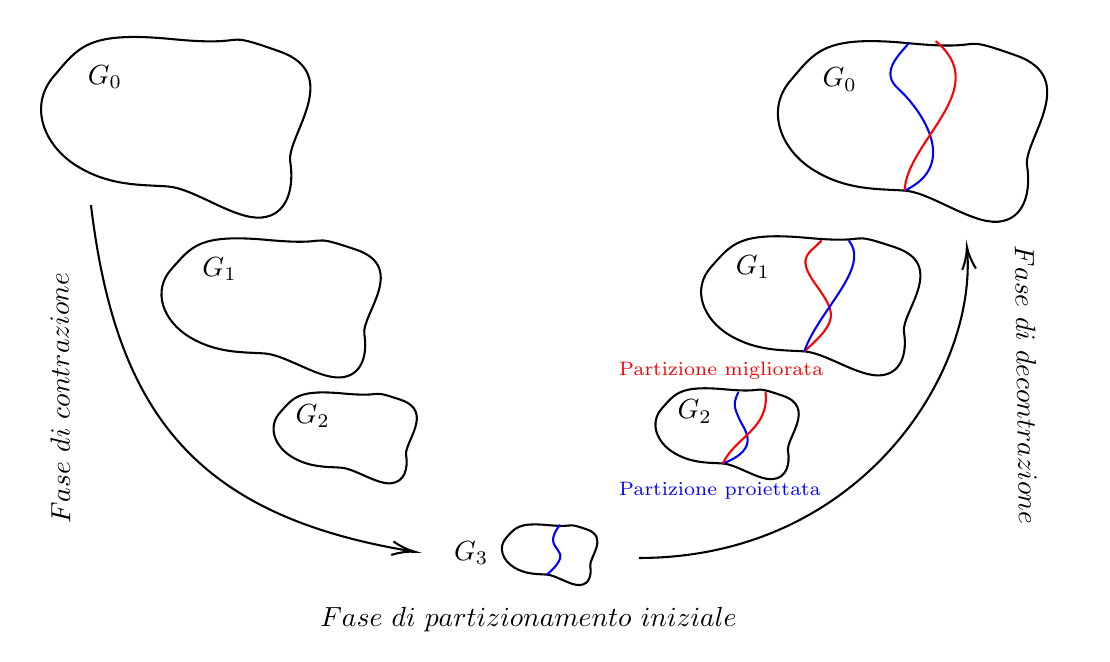
\begin{tikzpicture}[x=0.75pt,y=0.75pt,yscale=-1,xscale=1]
%uncomment if require: \path (0,301); %set diagram left start at 0, and has height of 301

%Shape: Polygon Curved [id:ds5681990127641572]
\draw   (13,23) .. controls (25,9) and (29,1) .. (70,5) .. controls (111,9) and (91,0) .. (122,11) .. controls (153,22) and (125.09,51.89) .. (127,64) .. controls (128.91,76.11) and (126,90) .. (113,91) .. controls (100,92) and (80.66,76.9) .. (68,76) .. controls (55.34,75.1) and (40,76) .. (24,66) .. controls (8,56) and (1,37) .. (13,23) -- cycle ;
%Shape: Polygon Curved [id:ds5791880784550985]
\draw   (69.88,115.65) .. controls (79.65,104.87) and (82.9,98.71) .. (116.29,101.79) .. controls (149.67,104.87) and (133.38,97.94) .. (158.63,106.41) .. controls (183.87,114.88) and (161.14,137.9) .. (162.7,147.22) .. controls (164.25,156.55) and (161.88,167.24) .. (151.3,168.01) .. controls (140.71,168.78) and (124.96,157.16) .. (114.66,156.46) .. controls (104.35,155.77) and (91.86,156.46) .. (78.83,148.76) .. controls (65.81,141.06) and (60.11,126.43) .. (69.88,115.65) -- cycle ;
%Shape: Polygon Curved [id:ds8471099289598505]
\draw   (122.17,184.81) .. controls (128.56,177.76) and (130.68,173.74) .. (152.5,175.75) .. controls (174.32,177.76) and (163.67,173.23) .. (180.17,178.77) .. controls (196.67,184.3) and (181.81,199.34) .. (182.83,205.44) .. controls (183.85,211.53) and (182.3,218.52) .. (175.38,219.02) .. controls (168.46,219.53) and (158.17,211.93) .. (151.44,211.48) .. controls (144.7,211.02) and (136.54,211.48) .. (128.02,206.44) .. controls (119.51,201.41) and (115.79,191.85) .. (122.17,184.81) -- cycle ;
%Shape: Polygon Curved [id:ds042557391147138635]
\draw   (231.1,245.21) .. controls (235.36,240.51) and (236.78,237.83) .. (251.33,239.17) .. controls (265.87,240.51) and (258.78,237.49) .. (269.78,241.19) .. controls (280.78,244.88) and (270.87,254.91) .. (271.55,258.97) .. controls (272.23,263.04) and (271.2,267.7) .. (266.58,268.03) .. controls (261.97,268.37) and (255.11,263.3) .. (250.62,263) .. controls (246.13,262.69) and (240.68,263) .. (235,259.64) .. controls (229.32,256.29) and (226.84,249.91) .. (231.1,245.21) -- cycle ;
%Shape: Polygon Curved [id:ds19971791116540039]
\draw   (368,25) .. controls (380,11) and (384,3) .. (425,7) .. controls (466,11) and (446,2) .. (477,13) .. controls (508,24) and (480.09,53.89) .. (482,66) .. controls (483.91,78.11) and (481,92) .. (468,93) .. controls (455,94) and (435.66,78.9) .. (423,78) .. controls (410.34,77.1) and (395,78) .. (379,68) .. controls (363,58) and (356,39) .. (368,25) -- cycle ;
%Shape: Polygon Curved [id:ds6697871941207159]
\draw   (329.88,114.65) .. controls (339.65,103.87) and (342.9,97.71) .. (376.29,100.79) .. controls (409.67,103.87) and (393.38,96.94) .. (418.63,105.41) .. controls (443.87,113.88) and (421.14,136.9) .. (422.7,146.22) .. controls (424.25,155.55) and (421.88,166.24) .. (411.3,167.01) .. controls (400.71,167.78) and (384.96,156.16) .. (374.66,155.46) .. controls (364.35,154.77) and (351.86,155.46) .. (338.83,147.76) .. controls (325.81,140.06) and (320.11,125.43) .. (329.88,114.65) -- cycle ;
%Shape: Polygon Curved [id:ds6317966254041107]
\draw   (306.17,182.81) .. controls (312.56,175.76) and (314.68,171.74) .. (336.5,173.75) .. controls (358.32,175.76) and (347.67,171.23) .. (364.17,176.77) .. controls (380.67,182.3) and (365.81,197.34) .. (366.83,203.44) .. controls (367.85,209.53) and (366.3,216.52) .. (359.38,217.02) .. controls (352.46,217.53) and (342.17,209.93) .. (335.44,209.48) .. controls (328.7,209.02) and (320.54,209.48) .. (312.02,204.44) .. controls (303.51,199.41) and (299.79,189.85) .. (306.17,182.81) -- cycle ;
%Curve Lines [id:da4556621139317687]
\draw [color={rgb, 255:red, 0; green, 0; blue, 255 }  ,draw opacity=1 ]   (250.62,263) .. controls (267,249) and (246,253) .. (257,239) ;
%Curve Lines [id:da3153745771749539]
\draw [color={rgb, 255:red, 0; green, 0; blue, 255 }  ,draw opacity=1 ]   (335.44,209.48) .. controls (355,202) and (345.05,192.39) .. (343.35,188.03) .. controls (341.65,183.68) and (339.62,181.49) .. (343,175) ;
%Curve Lines [id:da24590148322887484]
\draw [color={rgb, 255:red, 255; green, 0; blue, 0 }  ,draw opacity=1 ]   (335.44,209.48) .. controls (341.44,196.48) and (358,193) .. (356,175) ;
%Curve Lines [id:da8069367964557173]
\draw [color={rgb, 255:red, 255; green, 0; blue, 0 }  ,draw opacity=1 ]   (374.66,155.46) .. controls (391.66,140.46) and (390,137) .. (380,123) .. controls (370,109) and (378,108) .. (383,102) ;
%Curve Lines [id:da030698152549456736]
\draw [color={rgb, 255:red, 0; green, 0; blue, 255 }  ,draw opacity=1 ]   (374.66,155.46) .. controls (381.66,135.46) and (407,115) .. (396,102) ;
%Curve Lines [id:da9188529841976845]
\draw [color={rgb, 255:red, 0; green, 0; blue, 255 }  ,draw opacity=1 ]   (423,78) .. controls (451,65) and (429,37) .. (420,29) .. controls (411,21) and (420,13) .. (425,7) ;
%Curve Lines [id:da500049878186364]
\draw [color={rgb, 255:red, 255; green, 0; blue, 0 }  ,draw opacity=1 ]   (423,78) .. controls (424,54) and (466,29) .. (438,6) ;
%Curve Lines [id:da5337953441131338]
\draw    (31,85) .. controls (42.94,184.5) and (80.62,234.5) .. (185.42,251.74) ;
\draw [shift={(187,252)}, rotate = 189.11] [color={rgb, 255:red, 0; green, 0; blue, 0 }  ][line width=0.75]    (10.93,-3.29) .. controls (6.95,-1.4) and (3.31,-0.3) .. (0,0) .. controls (3.31,0.3) and (6.95,1.4) .. (10.93,3.29)   ;
%Curve Lines [id:da17376352225172775]
\draw    (295,255) .. controls (400.93,255) and (457.86,166.79) .. (453.16,106.81) ;
\draw [shift={(453,105)}, rotate = 84.29] [color={rgb, 255:red, 0; green, 0; blue, 0 }  ][line width=0.75]    (10.93,-3.29) .. controls (6.95,-1.4) and (3.31,-0.3) .. (0,0) .. controls (3.31,0.3) and (6.95,1.4) .. (10.93,3.29)   ;

% Text Node
\draw (28,16.4) node [anchor=north west][inner sep=0.75pt]    {$G_{0}$};
% Text Node
\draw (83.23,108.82) node [anchor=north west][inner sep=0.75pt]    {$G_{1}$};
% Text Node
\draw (128.13,179.36) node [anchor=north west][inner sep=0.75pt]    {$G_{2}$};
% Text Node
\draw (204.41,245.38) node [anchor=north west][inner sep=0.75pt]    {$G_{3}$};
% Text Node
\draw (382,17.4) node [anchor=north west][inner sep=0.75pt]    {$G_{0}$};
% Text Node
\draw (340.23,107.82) node [anchor=north west][inner sep=0.75pt]    {$G_{1}$};
% Text Node
\draw (312.13,177.36) node [anchor=north west][inner sep=0.75pt]    {$G_{2}$};
% Text Node
\draw (10.34,240.07) node [anchor=north west][inner sep=0.75pt]  [rotate=-269.56]  {$Fase\ di\ contrazione$};
% Text Node
\draw (486.92,102.91) node [anchor=north west][inner sep=0.75pt]  [rotate=-89.15]  {$Fase\ di\ decontrazione$};
% Text Node
\draw (140,277.4) node [anchor=north west][inner sep=0.75pt]    {$Fase\ di\ partizionamento\ iniziale$};
% Text Node
\draw (284,217) node [anchor=north west][inner sep=0.75pt]   [align=left] {{\scriptsize \textcolor[rgb]{0,0,1}{Partizione proiettata}}};
% Text Node
\draw (284,159) node [anchor=north west][inner sep=0.75pt]  [font=\normalsize] [align=left] {{\scriptsize \textcolor[rgb]{1,0,0}{Partizione migliorata}}};


\end{tikzpicture}

    \caption{Schema grafico del partizionamento multi-livello}
    \label{fig:multi-level-graph-partitioning}
\end{figure}

L'approccio multi-livello per la partizione di grafi si articola in tre fasi principali:
\begin{enumerate}
    \item \textbf{Fase di contrazione} (\textit{contraction/coarsening phase}):
    si crea una gerarchia di grafi riducendo iterativamente la dimensione del grafo iniziale.
    Questo viene fatto comunemente individuando e contraendo coppie di nodi adiacenti, ovvero individuando un
    sottoinsieme degli archi del grafo da contrarre, $M \subseteq E $ detti \textit{match}.
    Si noti che la scelta di contrarre coppie di nodi adiacenti porta a grafi grossolani i cui nodi rappresentano
    sottografi del grafo iniziale densamente connessi.
    In base allo specifico problema, una determinata funzione di \textit{rating} classifica gli archi individuando
    quale sottoinsieme degli archi $E$ debba essere assegnato ad $M$ affinch\`e la somma dei \textit{rating} degli in
    $M$ sia globalmente massimizzata.
    Si consideri che un nodo gi\`a contratto non pu\`o essere pi\`u coinvolto in un ulteriore \textit{matching}
    allo stesso livello della gerarchia.
    \item \textbf{Fase di partizionamento iniziale} (\textit{initial partitioning phase}): quando a seguito delle
    contrazioni il grafo risulta essere di ordine abbastanza piccolo, in relazione ad un qualche threshold,
    esso pu\`o essere partizionato direttamente con algoritmi costosi, fornendo una partizione iniziale sul grafo
    pi\`u grossolano della gerarchia.
    \item \textbf{Fase di decontrazione} (\textit{refinement/uncoarsening phase}), i matching vengono iterativamente
    decontratti, e i relativi nodi vengono associati a blocchi della partizione del grafo pi\`u grossolano,
    proiettandola sul grafo pi\`u raffinato.
    Per fare in modo che la partizione al livello pi\`u grossolano tenga conto delle sotto-strutture ai livelli
    pi\`u raffinati, un algoritmo di miglioramento locale (\textit{local improvement}) ricolloca i nodi tra i
    blocchi per migliorare la dimensione del taglio o l'equilibrio delle dimensioni tra i blocchi.
\end{enumerate}




